% !TeX spellcheck = it_IT
\newpage
\section{Descrizione del dominio}
Per monitorare l'inquinamento urbano, ogni \textbf{area di rilevamento} ha un nome e contiene un certo numero di \textbf{sensori} (può essere 0 se non sono ancora stati impostati), dove ciascuno misura almeno un \textbf{parametro} ambientale in una certa unità di misura che ha nome e descrizione. Un sensore può effettuare varie \textbf{misurazioni} riguardanti uno dei suoi parametri, segnando la data, l'ora e il valore misurato.\\

Per ogni \textbf{utente} interessa il Codice Fiscale, nome e cognome, la data di nascita, il telefono e l'indirizzo. Un utente \textbf{cittadino} può inviare più \textbf{segnalazioni} con un titolo, una descrizione e la data, riguardante una possibile fonte inquinante. Un utente \textbf{responsabile locale} può supervisionare un area di rilevamento (ogni area di rilevamento ha un responsabile), può approvare le fonti inquinanti precedentemente proposte da un cittadino e può proporre degli interventi di mitigazione. Un utente \textbf{amministratore} può approvare gli interventi proposti dai responsabili e gestire delle soglie. Ogni \textbf{soglia} è definita da un massimo e un minimo e riguarda un parametro ambientale.\\

Di una \textbf{fonte inquinante} interessa il livello stimato di impatto ambientale, latitudine e longitudine per definire la posizione precisa e se è stata approvata da un responsabile (e nel caso da quale responsabile). Ogni fonte inquinate ha un \textbf{tipo}, con un nome e una descrizione, e influenza almeno un'area di rilevamento.\\	

Degli \textbf{interventi di mitigazione} interessa la data di inizio e di fine, la priorità assegnata e la fattibilità. Un intervento può essere proposto da un responsabile locale o generato dal sistema. Un intervento  ha un \textbf{tipo}, con nome e descrizione, e è composto da almeno un \textbf{attività operativa}, definita da un nome e il tempo richiesto per la sua realizzazione. Sia interventi che attività operative hanno uno \textbf{stato} con nome e descrizione, ma hanno possibili stati diversi. Un attività operativa può essere in attesa di altre attività e richiede certe \textbf{risorse} in una certa quantità. Ogni risorsa ha un nome e si distingue tra \textbf{materiali} e \textbf{personale}, per i quali si segna relativamente il costo unitario e il costo giornaliero. Dalle risorse richieste per un'attività operativa si ricava il budget necessario per realizzarla.
Una risorsa viene fornita da una \textbf{azienda}, di cui interessa la denominazione, la partita IVA, l'indirizzo, l'email e il numero di telefono. In più ogni intervento viene incaricato ad un azienda principale.

\newpage
\section{Schema concettuale}
\begin{center}
	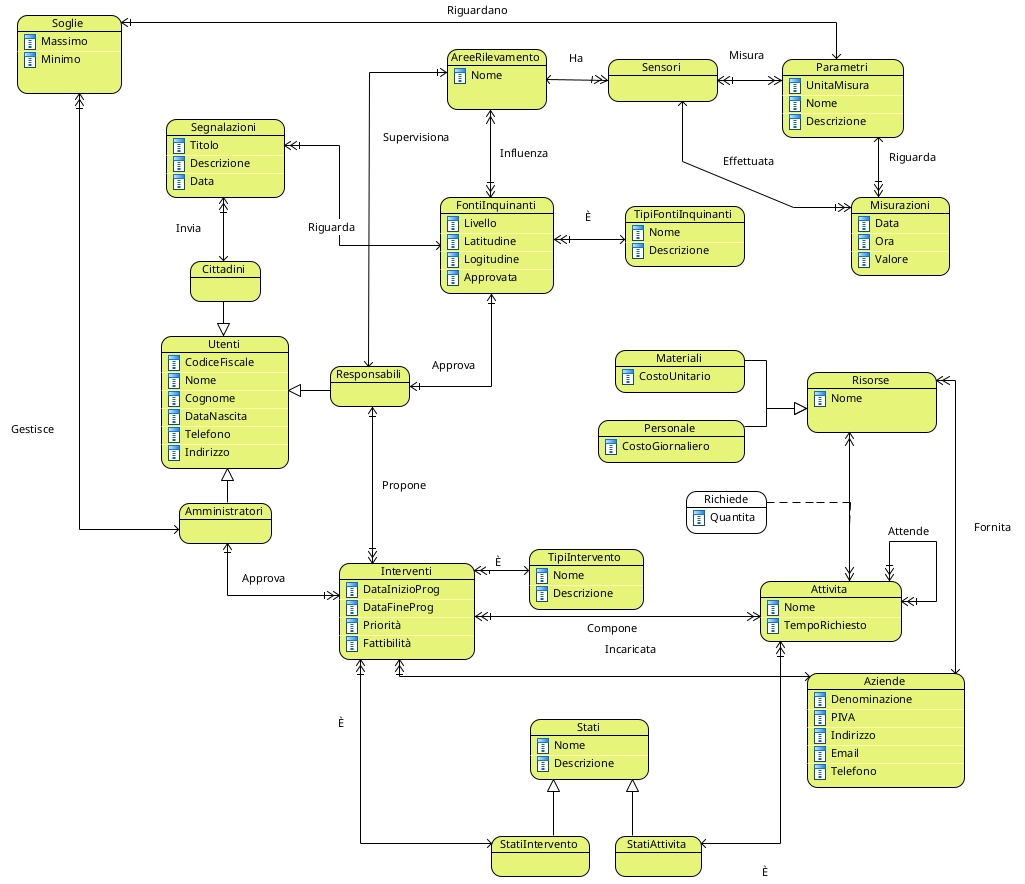
\includegraphics[scale=1.8]{BD0125_1.7.jpg}
\end{center}

\subsection{Vincoli}
\subsubsection{Interrelazionali}
I vincoli interrelazionali sono:
\begin{itemize}
	\item Un intervento per un'area può essere proposto solo dal responsabile di quell'area
\end{itemize}
\subsubsection{Intrarelazionali}
I vincoli intrarelazionali sono:
\begin{itemize}
	\item \textbf{Soglie}: $\text{Massimo} > \text{Minimo}$
	\item \textbf{Interventi}: $\text{DataInizio} < \text{DataFine}, \text{Priorita}\geq0, \text{Fattibilita}\geq0$
	\item \textbf{Fonti Inquinanti}: $\text{Livello}>0, -90 \leq \text{Latitudine} \leq 90, -90 \leq \text{Longitudine}\leq90$, \textit{Livello} è NULLABLE
	\item \textbf{Attività}: $\text{TempoRichiesto}>0$
	\item \textbf{Attende}: $\text{IdAttivita1} \neq \text{IdAttivita2}$
	\item \textbf{Materiale}: $\text{CostoUnitario}\geq0$
	\item \textbf{Personale}: $\text{CostoGiornaliero}\geq0$
	\item \textbf{Utenti}: \textit{Telefono} e \textit{Indirizzo} sono NULLABLE
	\item \textbf{TipoFontiInquinanti}: \textit{Descrizione} è NULLABLE
	\item \textbf{Stati}: \textit{Descrizione} è NULLABLE
\end{itemize}

\section{Schema logico relazionale}
\begin{center}
	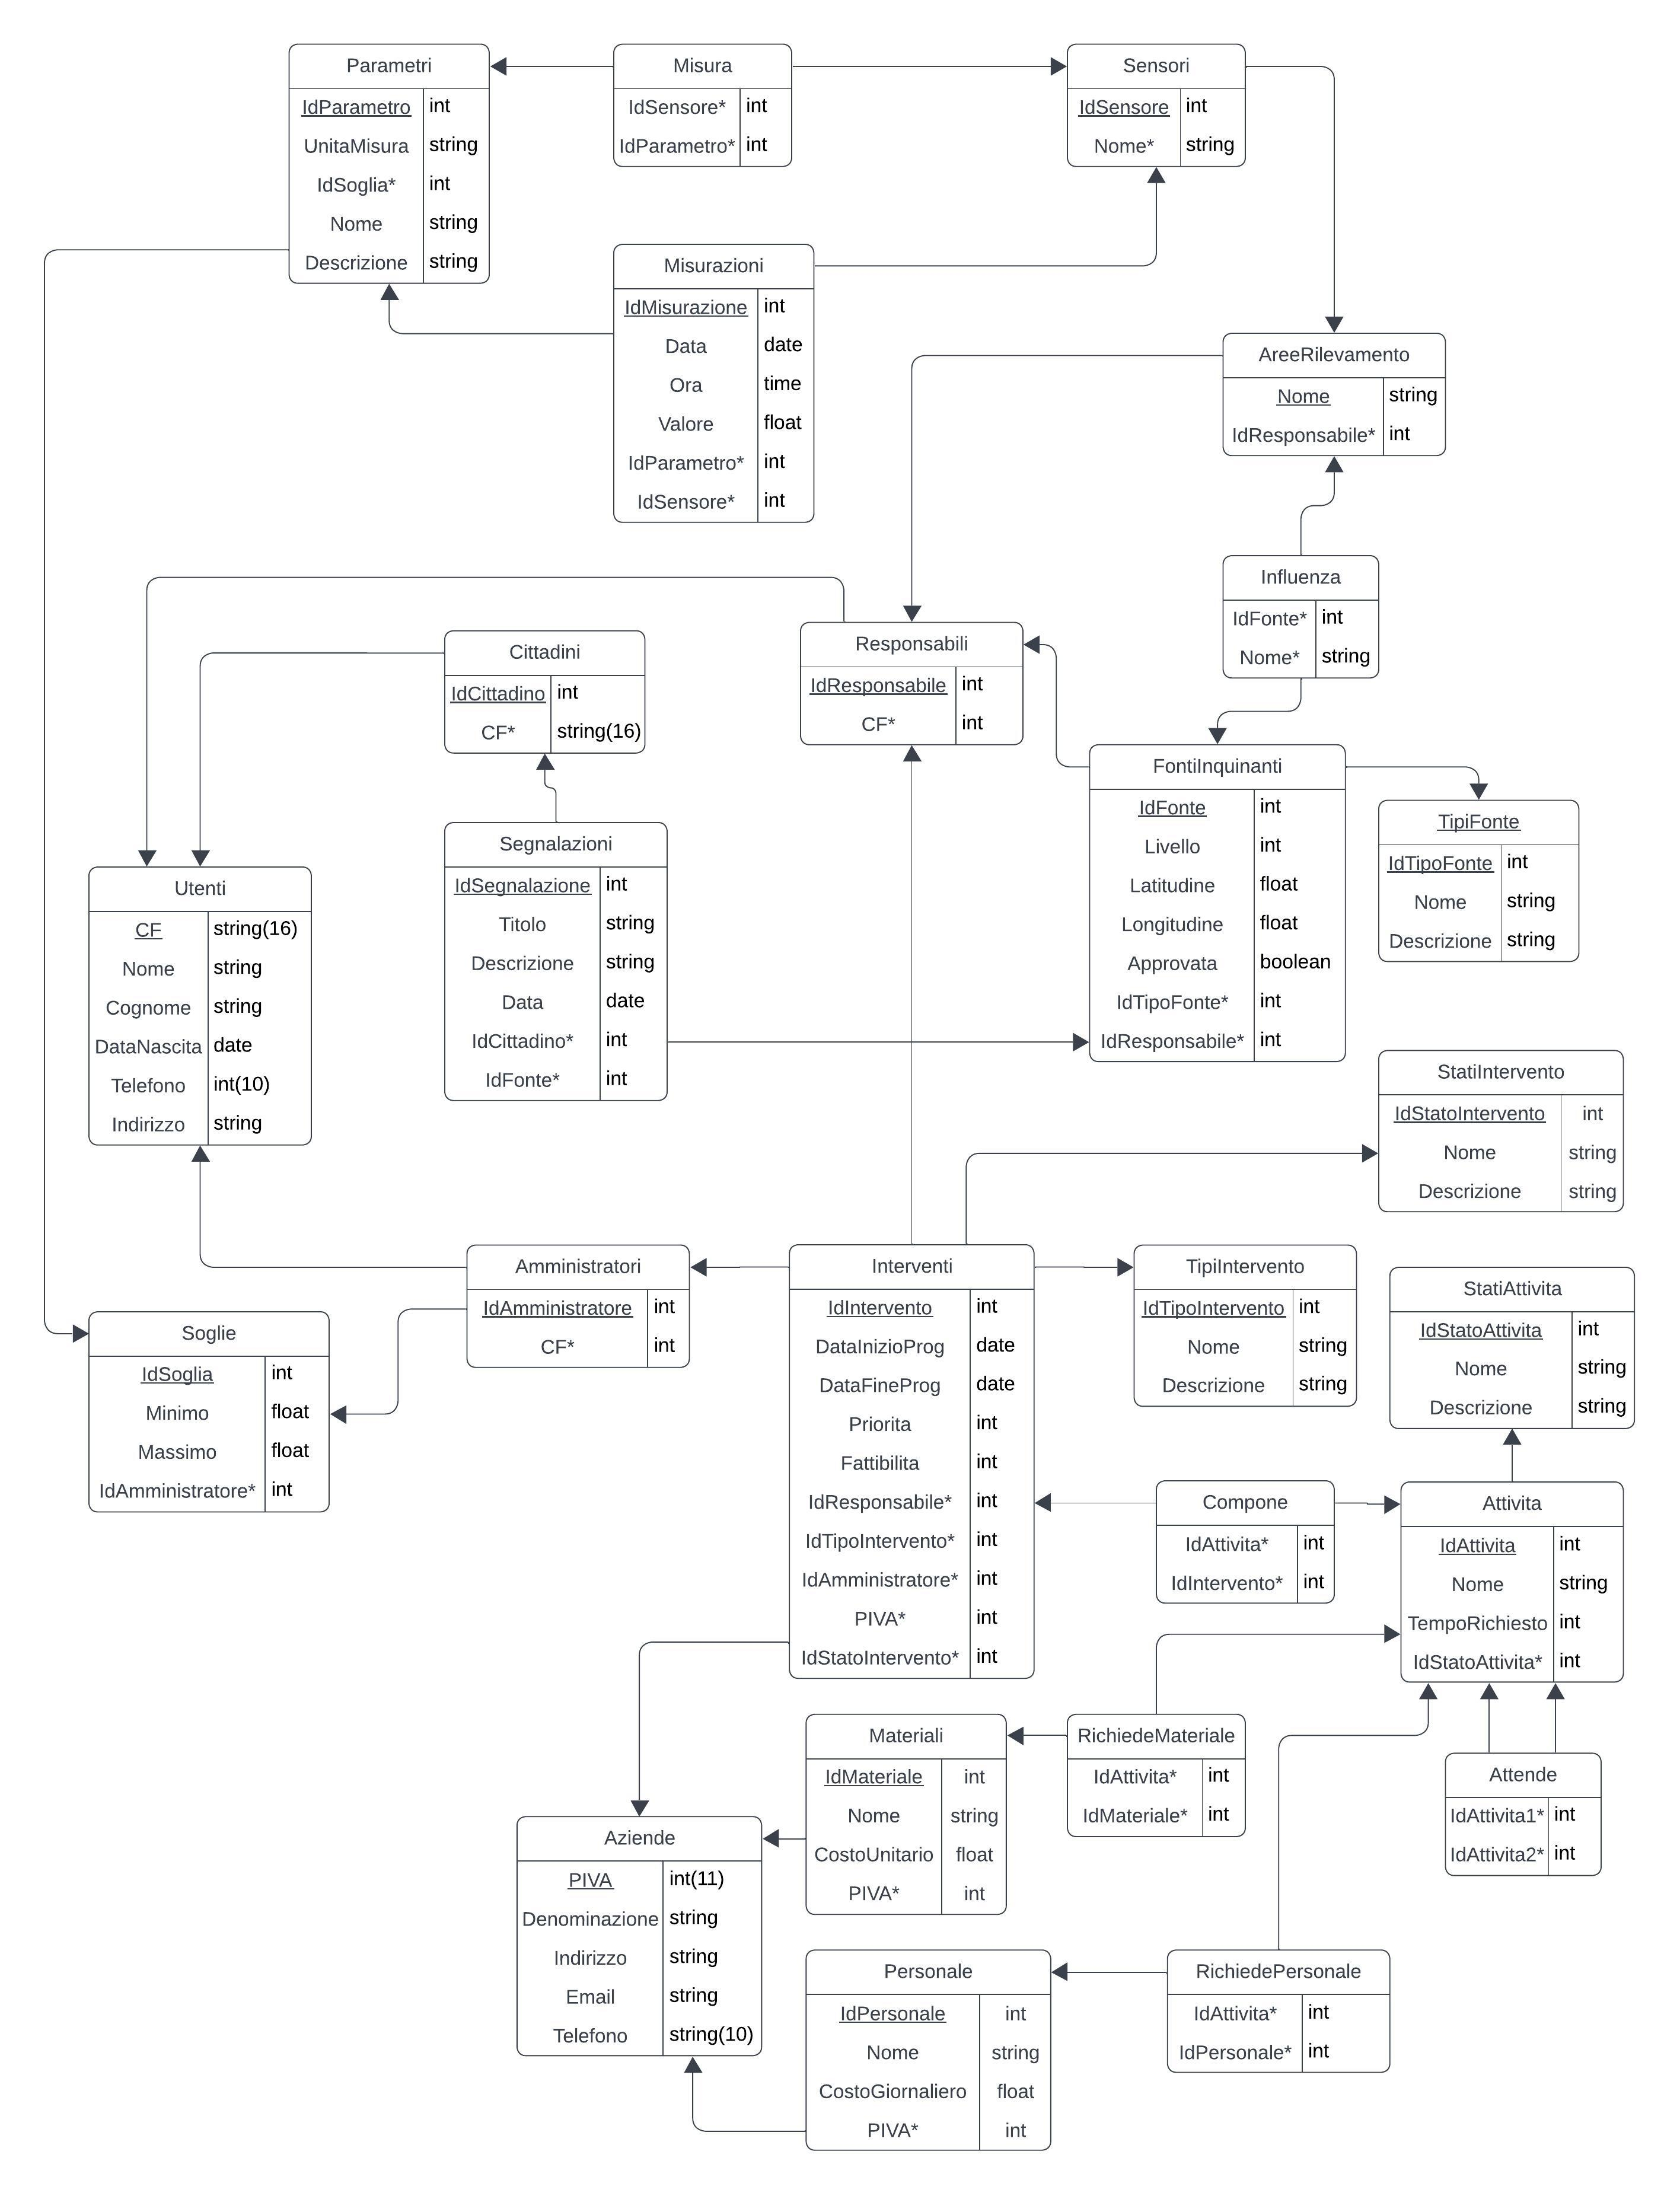
\includegraphics[scale=0.6]{BD0125_logico_1.6.jpeg}
\end{center}

\newpage
\subsection{Dipendenze funzionali}
Di seguito le dipendenze funzionali per ogni relazione:
\begin{itemize}
	\item \textbf{Utenti}
	\begin{equation*}
		\{\text{CF} \to \text{Nome}, \text{Cognome}, \text{DataNascita}, \text{Telefono}, \text{Indirizzo}\}
	\end{equation*}
	\item \textbf{Segnalazioni}
	\begin{equation*}
		\{\text{IdSegnalazione} \to \text{Titolo}, \text{Descrizione}, \text{Data}, \text{IdCittadino}, \text{IdFonte}\}
	\end{equation*}
	\item \textbf{Cittadino}
	\begin{equation*}
		\{\text{IdCittadino} \to \text{CF}\}
	\end{equation*}
	\item \textbf{Responsabili}
	\begin{equation*}
		\{\text{IdResponsabile} \to \text{CF}\}
	\end{equation*}
	\item \textbf{AreeRilevamento}
	\begin{equation*}
		\{\text{Nome} \to \text{IdResponsabile}\}
	\end{equation*}
	\item \textbf{FontiInquinanti}
	\begin{equation*}
		\{\text{IdFonte} \to \text{Livello}, \text{Latitudine}, \text{Longitudine}, \text{Approvata}, \text{IdTipoFonte}, \text{IdResponsabile}	\}
	\end{equation*}
	\item \textbf{TipiFonte}
	\begin{align*}
		& \{\text{IdTipoFonte} \to (\text{Nome}, \text{Descrizione}),\\
		& \text{Nome} \to (\text{IdTipoFonte}, \text{Descrizione}),\\
		& \text{Descrizione} \to (\text{IdTipoFonte}, \text{Nome})\}
	\end{align*}
	\item \textbf{StatiIntervento}
	\begin{align*}
		& \{\text{IdStatoIntervento} \to (\text{Nome}, \text{Descrizione}), \\
		& \text{Descrizione} \to (\text{IdStatoIntervento}, \text{Nome}),\\
		& \text{Nome} \to \text{IdStatoIntervento}, \text{Descrizione}\}
	\end{align*}
	\item \textbf{Sensori}
	\begin{equation*}
		\{\text{IdSensore} \to \text{IdArea}\}
	\end{equation*}
	\item \textbf{Misurazioni}
	\begin{align*}
		& \{\text{IdMisurazione} \to (\text{Data}, \text{Ora}, \text{Valore}, \text{IdParametro}, \text{IdSensore}),\\
		& \text{IdParametro}, \text{IdSensore}, \text{Data}, \text{Ora} \to (\text{Valore}, \text{IdMisurazione})\}
	\end{align*}
	\item \textbf{Parametri}
	\begin{equation*}
		\{\text{IdParametro} \to \text{UnitaMisura},\text{Nome}, \text{Descrizione}, \text{IdSoglia}\}
	\end{equation*}
	\item \textbf{Soglie}
	\begin{equation*}
		\{\text{IdSoglia}->\text{Minimo}, \text{Massimo}, \text{IdAmministratore}\}
	\end{equation*}
	\item \textbf{Amministratori}
	\begin{equation*}
		\{\text{IdAmministratore}\to\text{CF}\}
	\end{equation*}
	\item \textbf{Interventi}
	\begin{align*}
		&\{\text{IdIntervento}\to\text{DataInizioProg}, \text{DataFineProg}, \text{Priorita}, \text{Fattibilita},\\ &\text{IdResponsabile}, \text{IdTipoIntervento}, \text{IdAmministratore}, \text{PIVA}, \text{IdStatoIntervento}\}
	\end{align*}
	\item \textbf{TipiIntervento}
	\begin{equation*}
		\{\text{IdTipoIntervento}\to\text{Nome}, \text{Descrizione}\}
	\end{equation*}
	\item \textbf{StatiAttivita}
	\begin{equation*}
		\{\text{IdStatoAttivita}\to\text{Nome}, \text{Descrizione}\}
	\end{equation*}
	\item \textbf{Attivita}
	\begin{equation*}
		\{\text{IdAttivita}\to\text{Nome}, \text{TempoRichiesto}, \text{IdStatoAttivita}\}
	\end{equation*}
	\item \textbf{Aziende}
	\begin{equation*}
		\{\text{PIVA}\to\text{Denominazione}, \text{Indirizzo}, \text{Email}, \text{Telefono}\}
	\end{equation*}
	\item \textbf{Personale}
	\begin{equation*}
		\{\text{IdPersonale}\to\text{Nome}, \text{CostoGiornaliero}, \text{PIVA}\}
	\end{equation*}
	\item \textbf{Materiali}
	\begin{equation*}
		\{\text{IdMateriale}\to\text{Nome}, \text{CostoUnitario}, \text{PIVA}\}
	\end{equation*}
\end{itemize}
\subsection{BCNF}
Tutte le relazioni sono in BCNF.

\section{Interrogazioni in SQL}
Di seguito le sei interrogazioni richieste:
\begin{enumerate}
	\item[a.] Il parametro e il valore delle misurazioni effettuate il 1 gennaio alle 18:00.
	\begin{lstlisting}[language=SQL]
		SELECT Parametri.Nome, Misurazioni.Valore
		FROM Misurazioni JOIN Parametri ON Parametri.IdParametro = Misurazioni.IdParametro
		WHERE Misurazioni.Data = '2025-01-01' AND Misurazioni.Ora = '18:00'
	\end{lstlisting}
	\item[b.] Numero di misurazioni fatte ogni giorno nel 2025 (con più di 5 misurazioni), ordinate per data.
	\begin{lstlisting}[language=SQL]
		SELECT Data, COUNT(*) AS NumeroMisurazioni
		FROM Misurazioni
		WHERE Data >= '01.01.2025'
		GROUP BY Data
		HAVING COUNT(*) > 5
		ORDER BY Data
	\end{lstlisting} 
	\item[c.] Livello medio delle fonti approvate per ogni tipo che ha più di 2 fonti.
	\begin{lstlisting}[language=SQL]
		SELECT T.Nome, AVG(F.Livello) AS LivelloMedio
		FROM FontiInquinanti F JOIN TipiFonte T ON F.IdTipoFonte = T.IdTipoFonte
		WHERE F.Approvata = true
		GROUP BY T.Nome
		HAVING COUNT(*) > 2
	\end{lstlisting} 
	\item[d.] Trova il nome e il tempo richiesto delle attività che hanno richiesto almeno un materiale.
	\begin{lstlisting}[language=SQL]
		SELECT Nome, TempoRichiesto
		FROM Attivita A
		WHERE EXISTS (
			SELECT *
			FROM RichiedeMateriale RM
			WHERE RM.IdAttivita = A.IdAttivita
		);
	\end{lstlisting} 
	\item[e.] Trova le aree di rilevamento in cui tutti i sensori presenti in quell'area misurano almeno un parametro. 
	\begin{lstlisting}[language=SQL]
		SELECT ar.Nome
		FROM AreeRilevamento ar
		WHERE NOT EXISTS (
			SELECT s.IdSensore
			FROM Sensori s
			WHERE s.Nome = ar.Nome
			AND NOT EXISTS (
				SELECT m.IdParametro
				FROM Misura m
				WHERE m.IdSensore = s.IdSensore
			)
		);
	\end{lstlisting} 
	\item[f.] Trova i responsabili il cui numero di interventi pianificati è maggiore del numero medio di interventi pianificati da tutti i responsabili.
	\begin{lstlisting}[language=SQL]
		SELECT IdResponsabile
		FROM Responsabili R
		WHERE (
			SELECT COUNT(*)
			FROM Interventi I
			WHERE I.IdResponsabile = R.IdResponsabile
		) > (
			SELECT AVG(TotaleInterventi)
			FROM (
				SELECT COUNT(*) AS TotaleInterventi
				FROM Interventi
				GROUP BY IdResponsabile
			) SubQuery
		);
	\end{lstlisting} 
\end{enumerate}

\section{Piani di accesso}
\begin{enumerate}
	\item[I.] Piani di accesso \textbf{logico}
	\begin{figure}[!h]
		\centering
		\begin{minipage}{.3\textwidth}
			\centering
			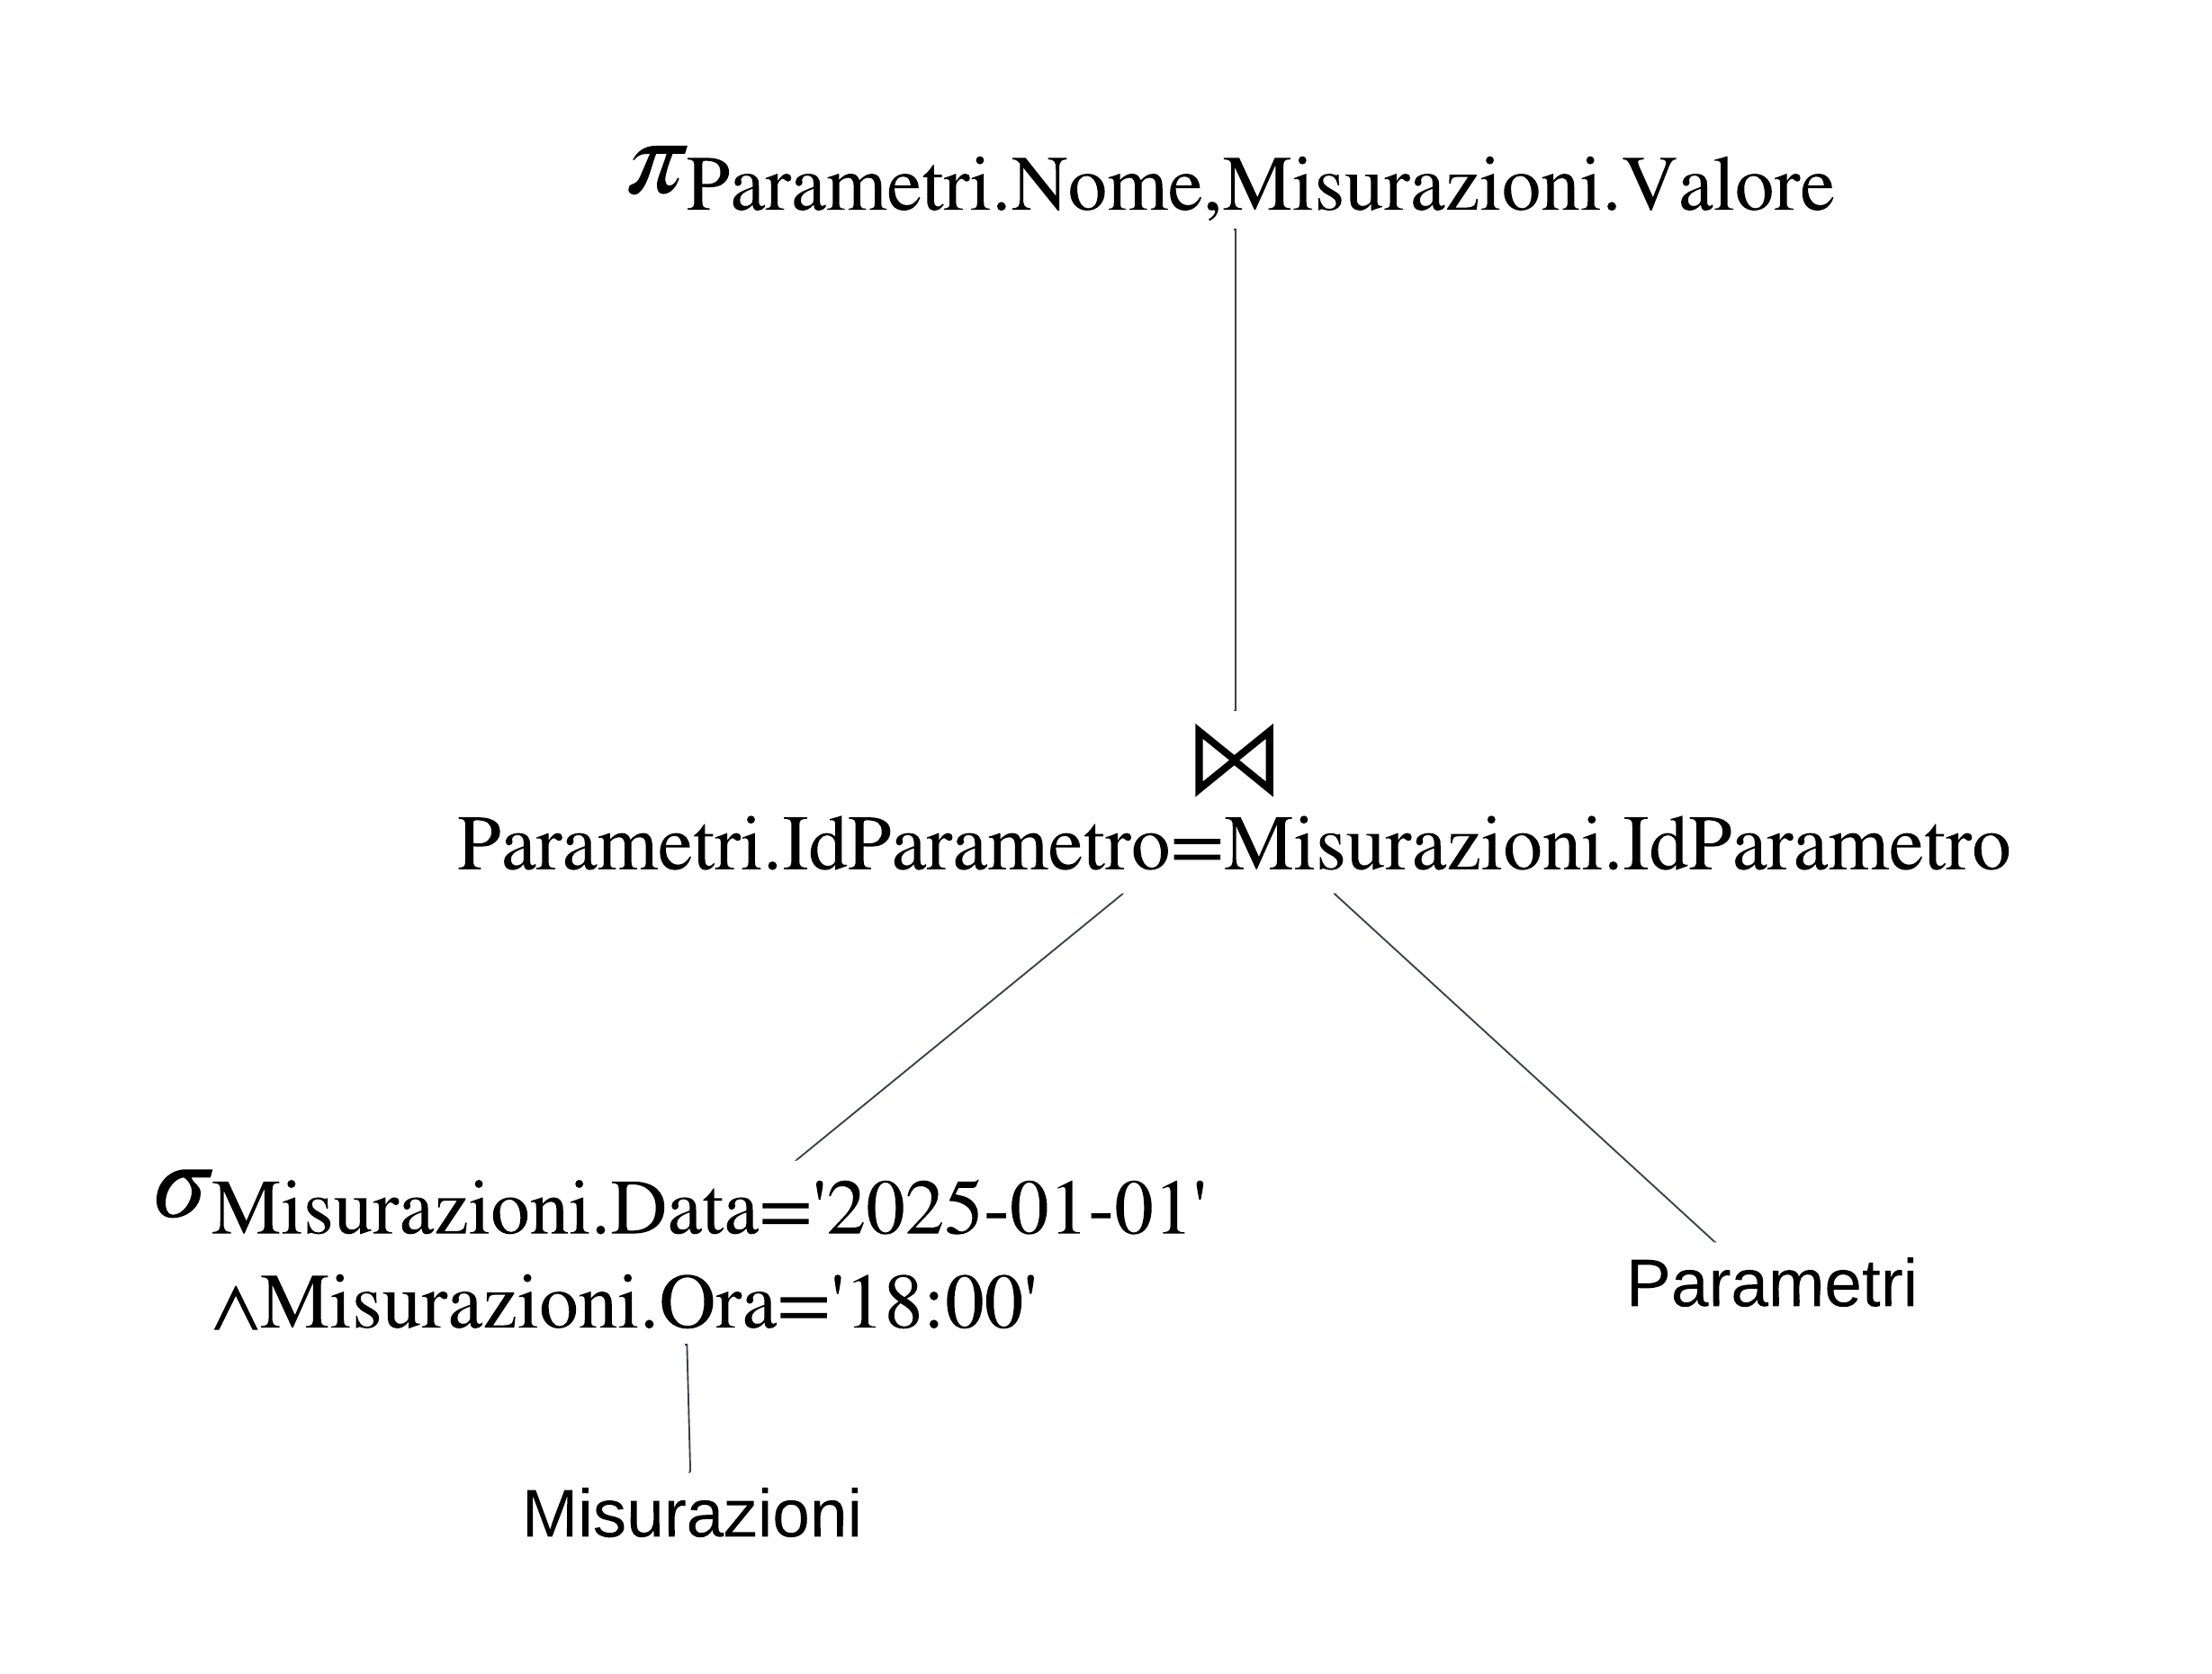
\includegraphics[scale=0.25]{1a.png}
			\captionof{figure}{Query \textit{a}}
		\end{minipage}
		\begin{minipage}{.3\textwidth}
			\centering
			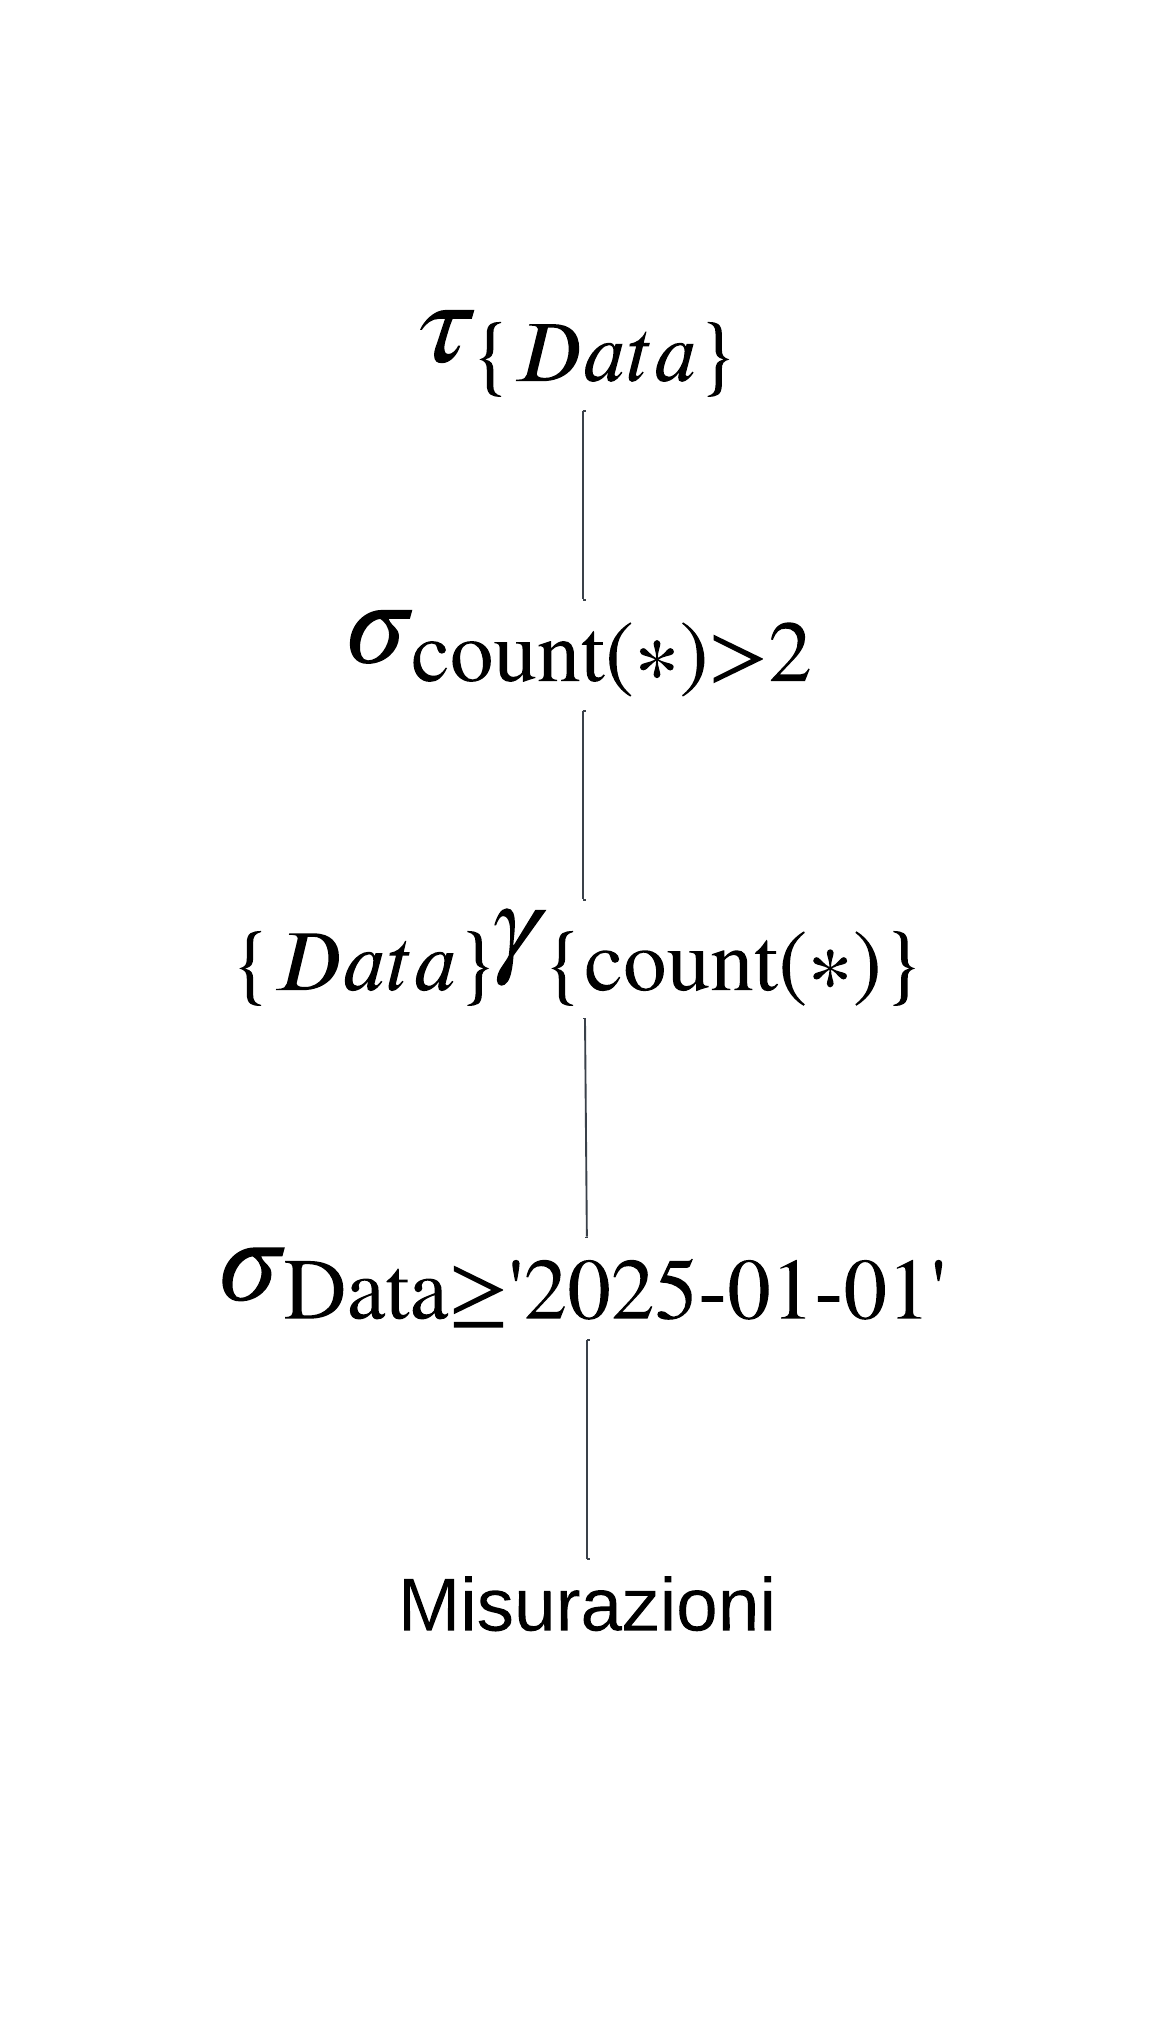
\includegraphics[scale=0.25]{1b.png}
			\captionof{figure}{Query \textit{b}}
		\end{minipage}
		\begin{minipage}{.3\textwidth}
			\centering
			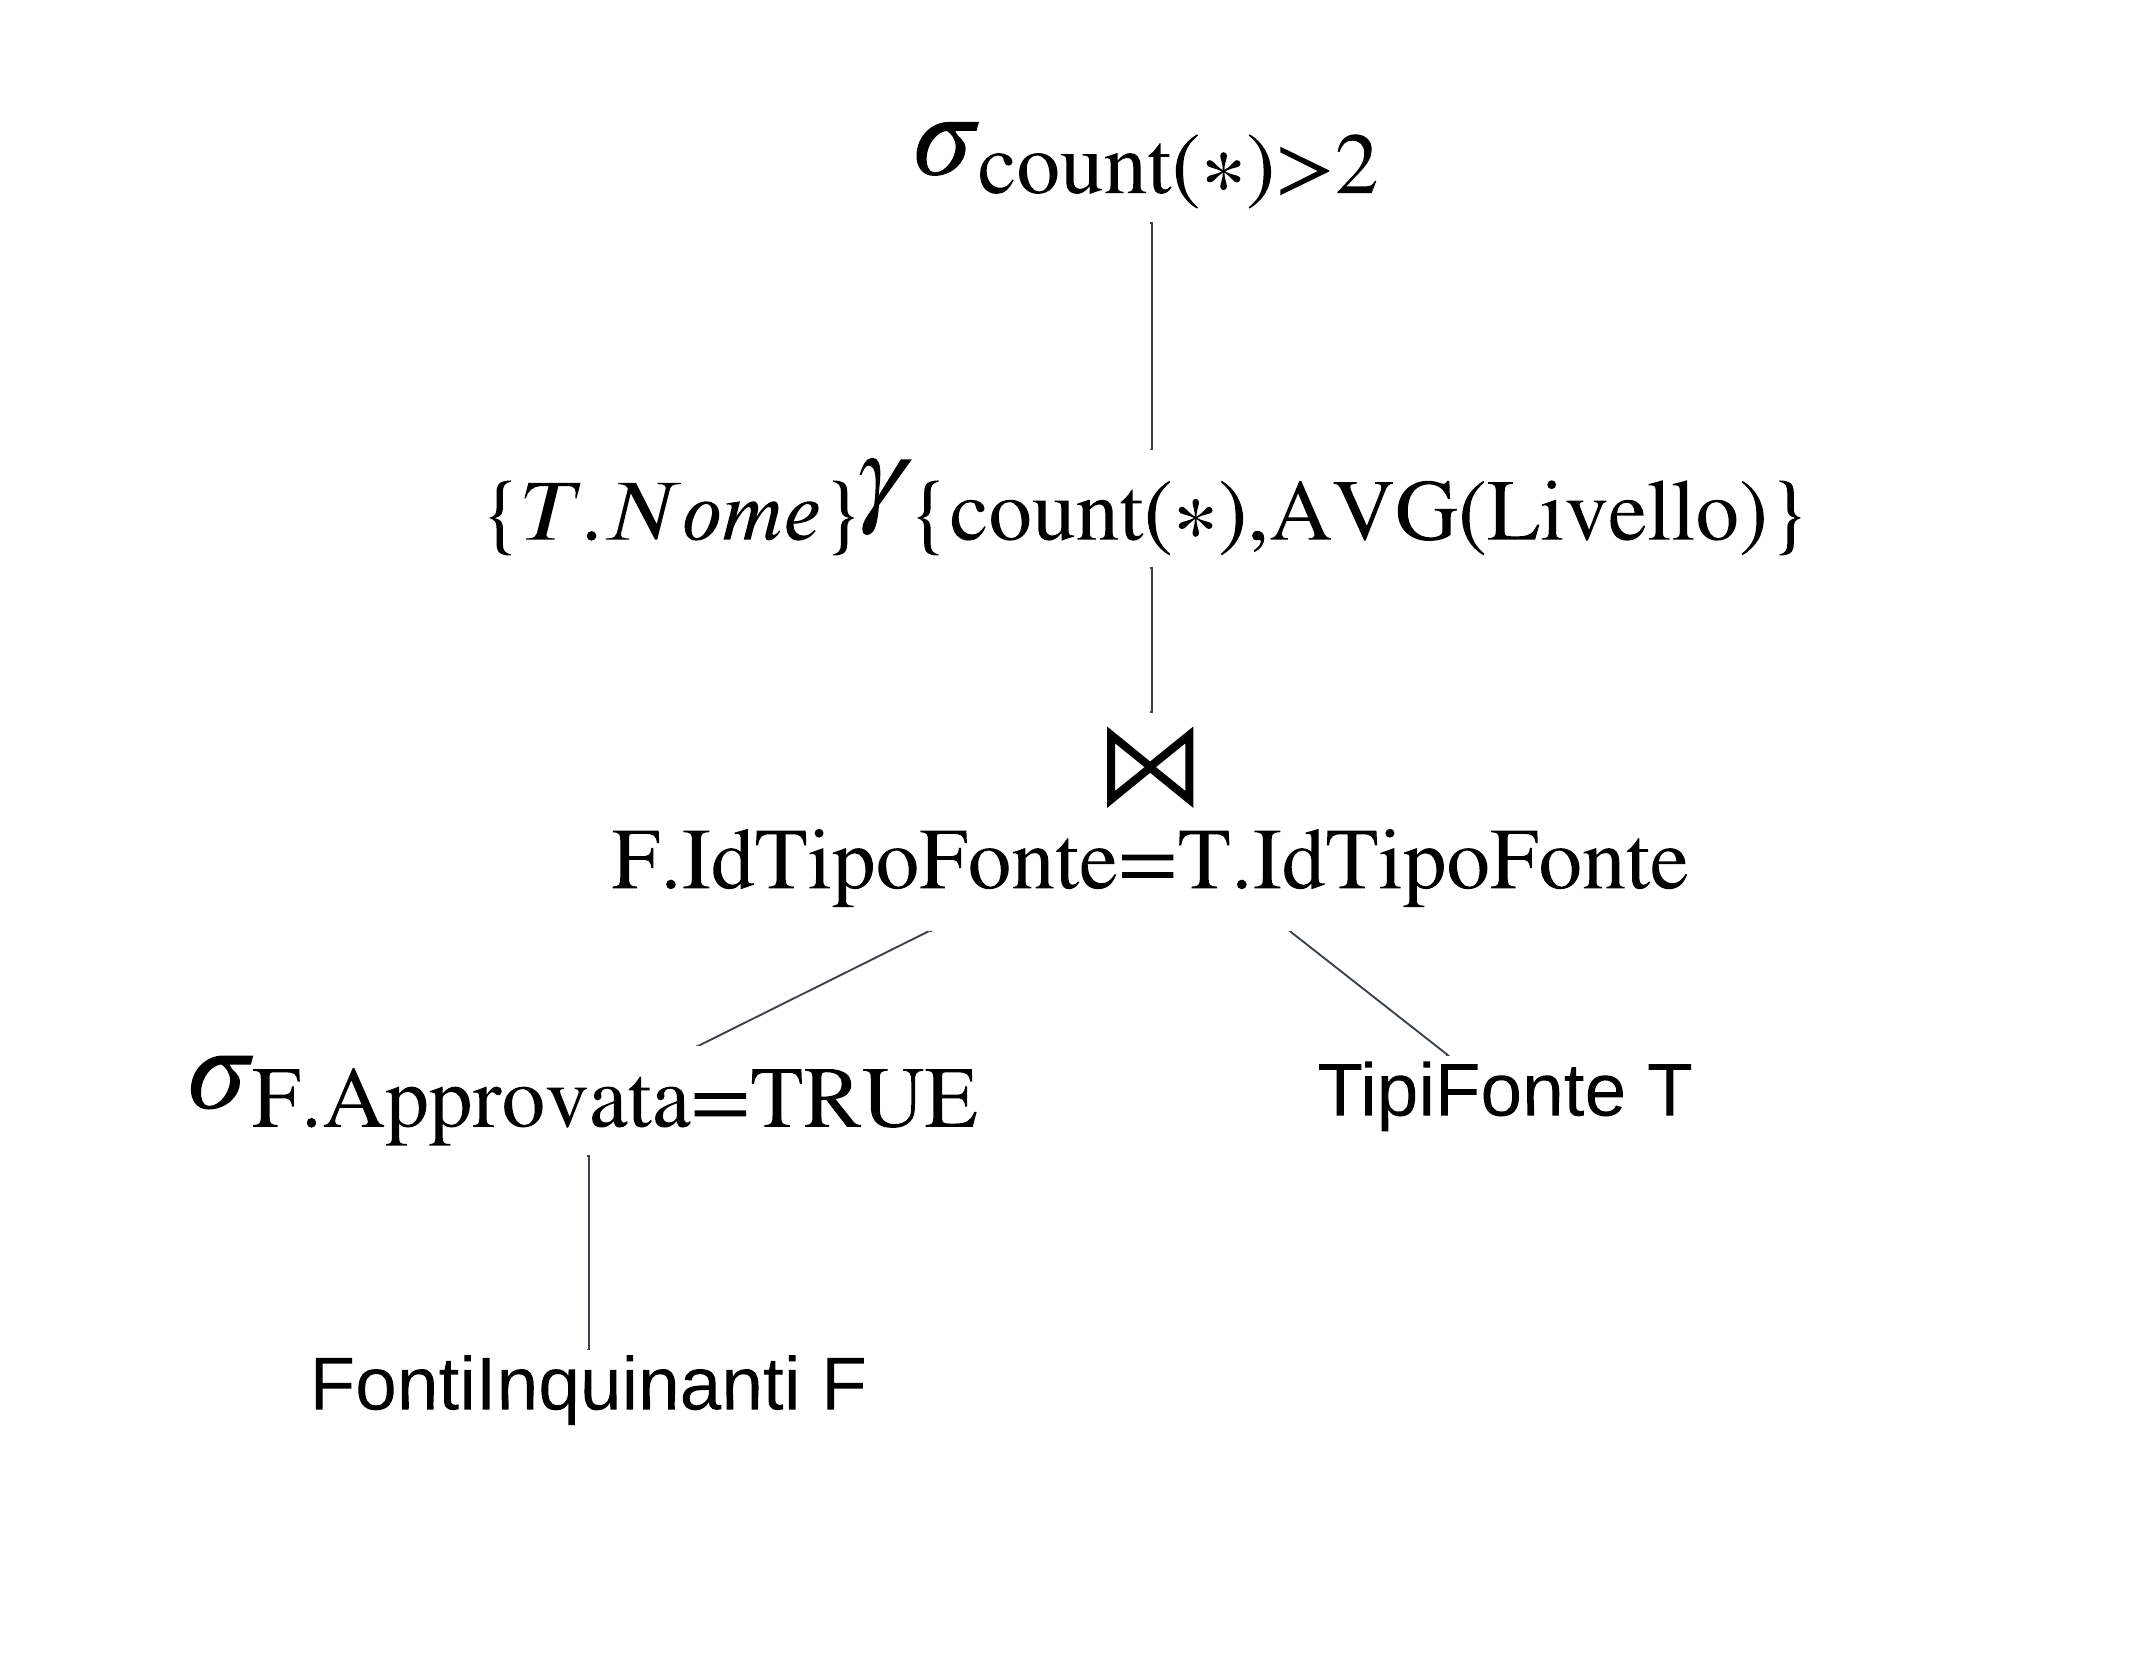
\includegraphics[scale=0.25]{1c.png}
			\captionof{figure}{Query \textit{c}}
		\end{minipage}
	\end{figure}
	\newpage
	\item[II.] Piani di accesso \textbf{fisico} senza uso di indici
	\begin{figure}[!h]
		\centering
		\begin{minipage}{.3\textwidth}
			\centering
			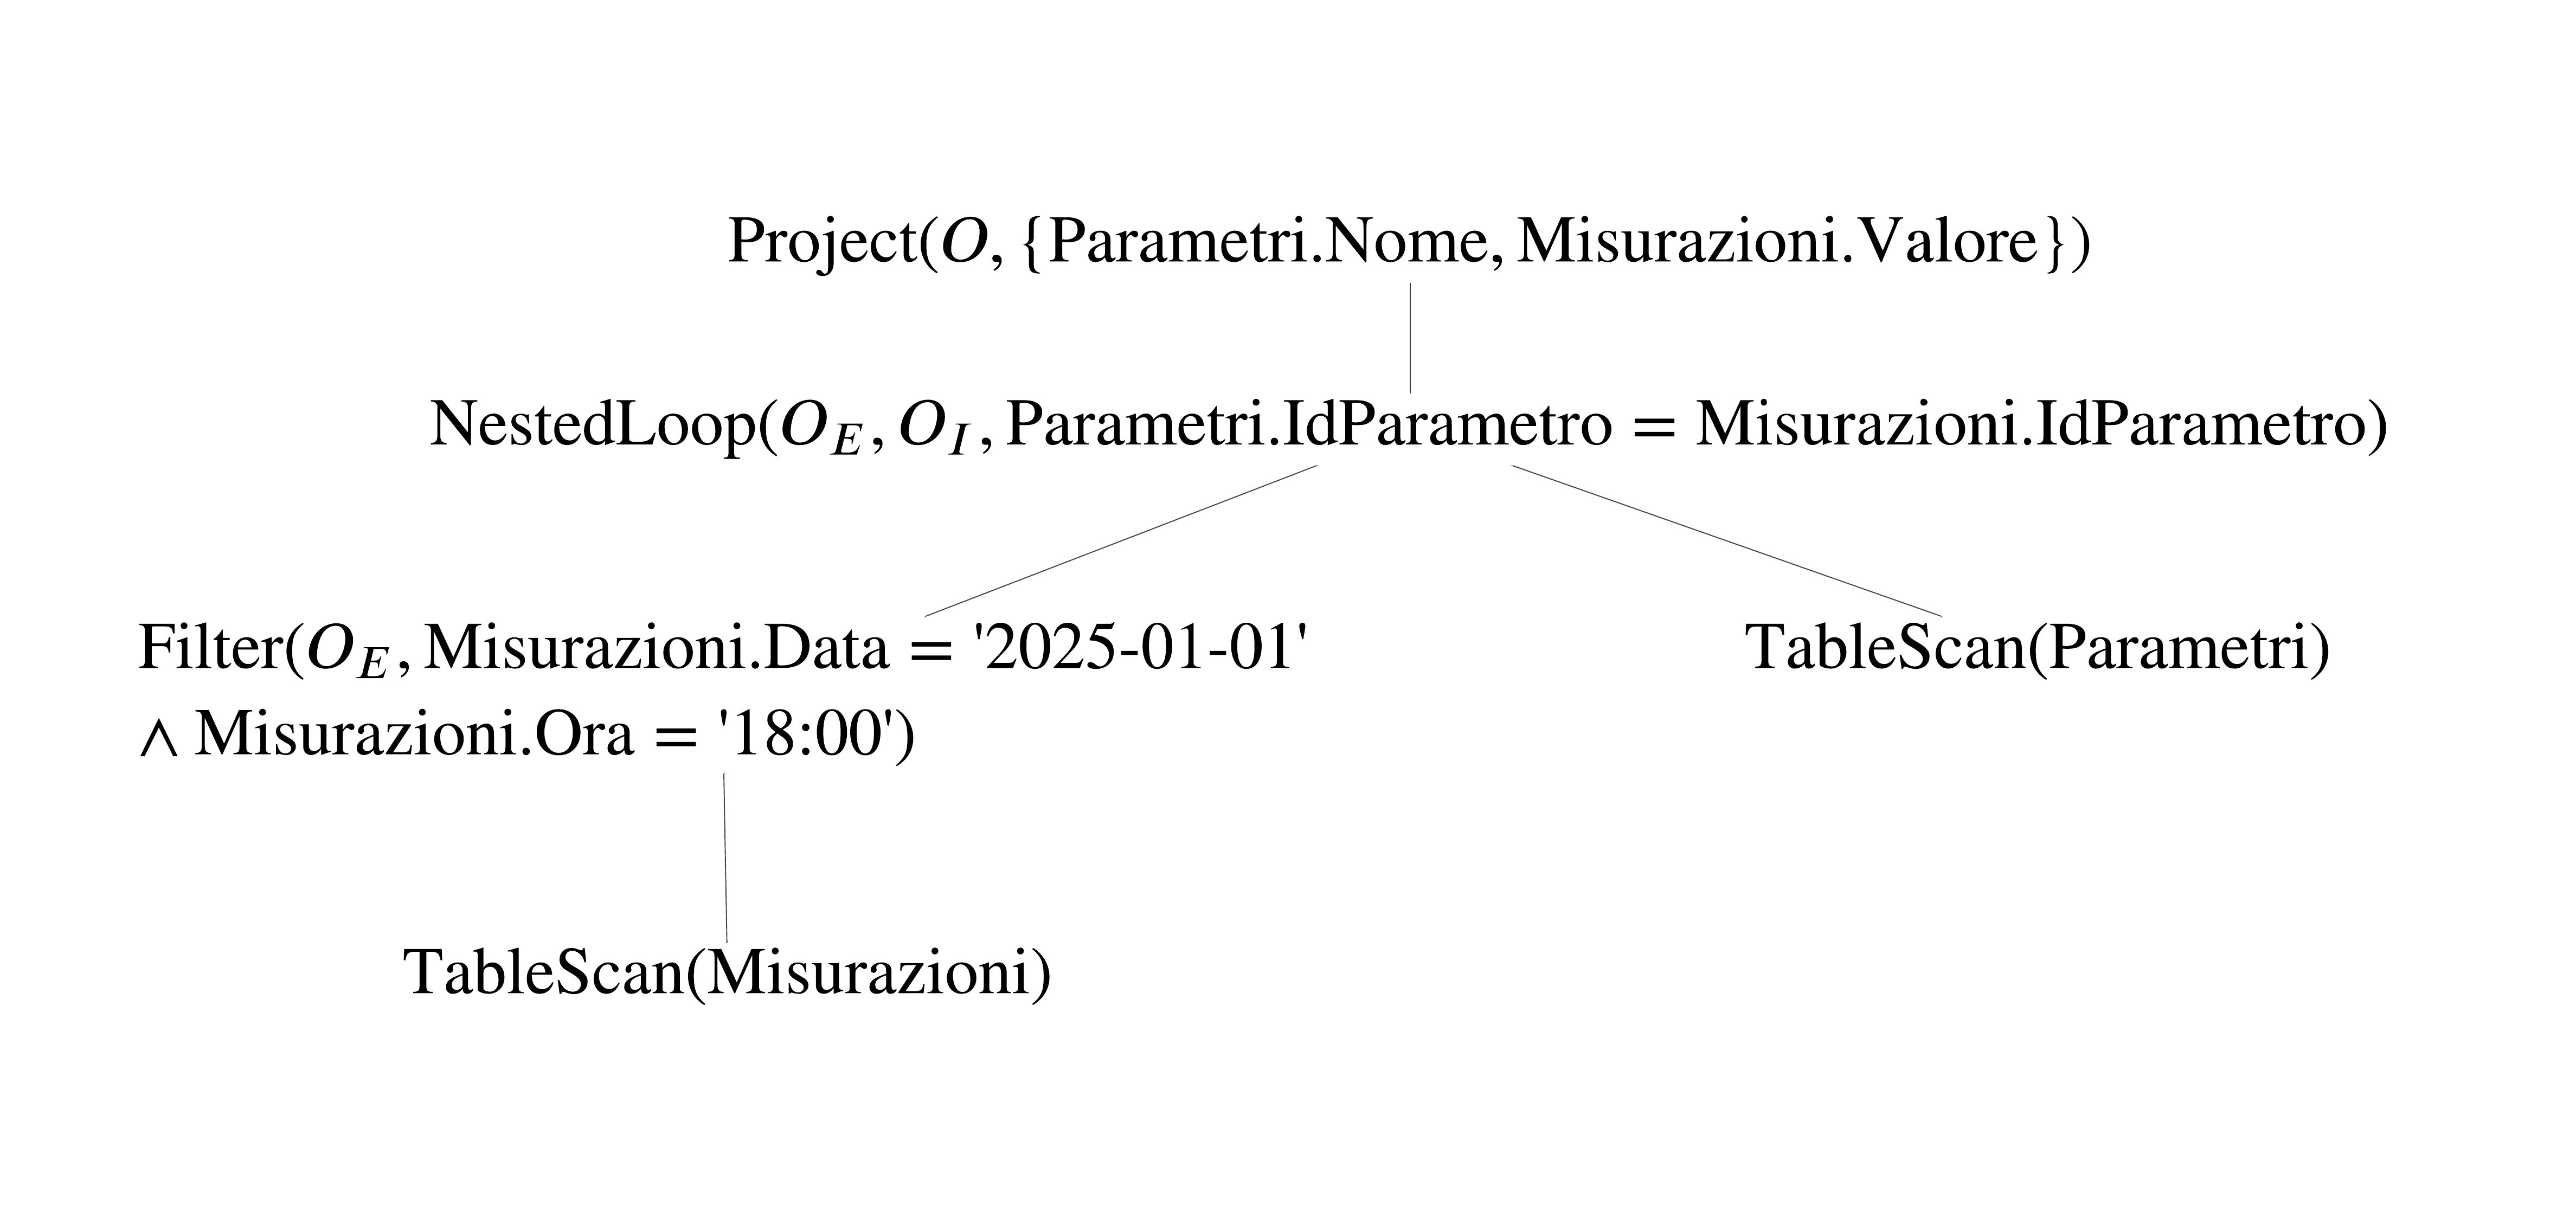
\includegraphics[scale=0.2]{2a.png}
			\captionof{figure}{Query \textit{a}}
		\end{minipage}\\
		\begin{minipage}{.3\textwidth}
			\centering
			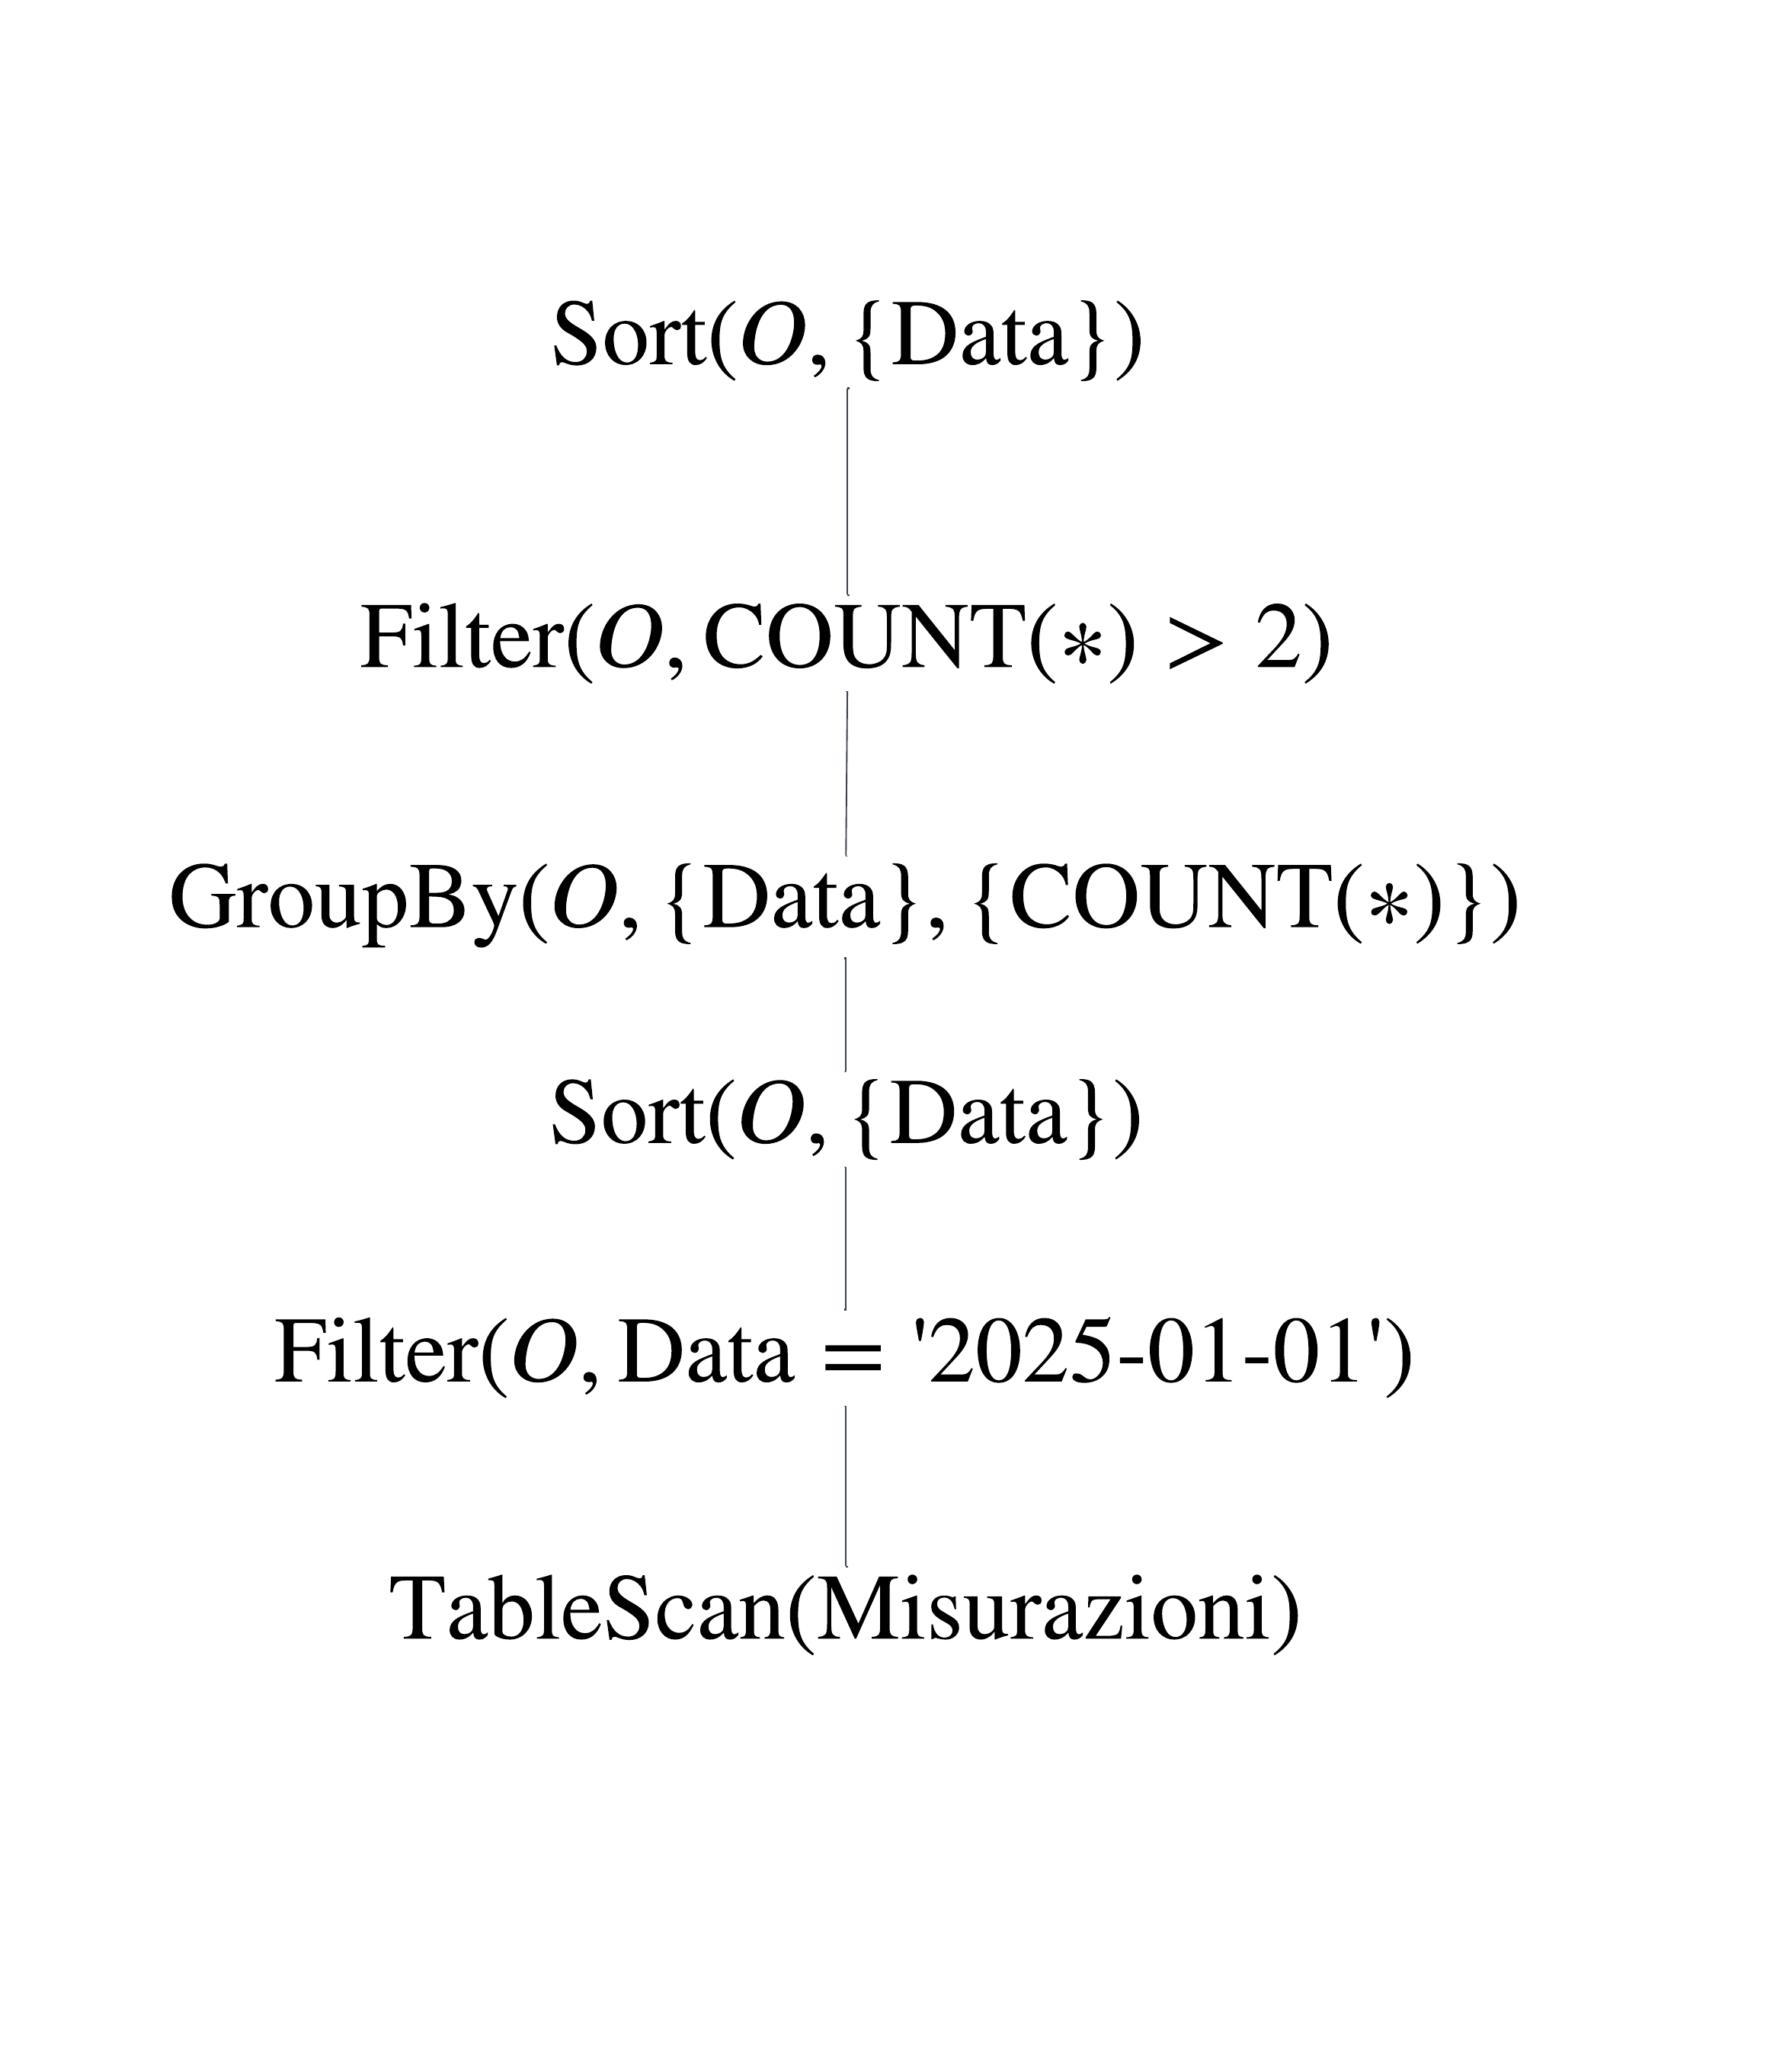
\includegraphics[scale=0.2]{2b.png}
			\captionof{figure}{Query \textit{b}}
		\end{minipage}
		\begin{minipage}{.3\textwidth}
			\centering
			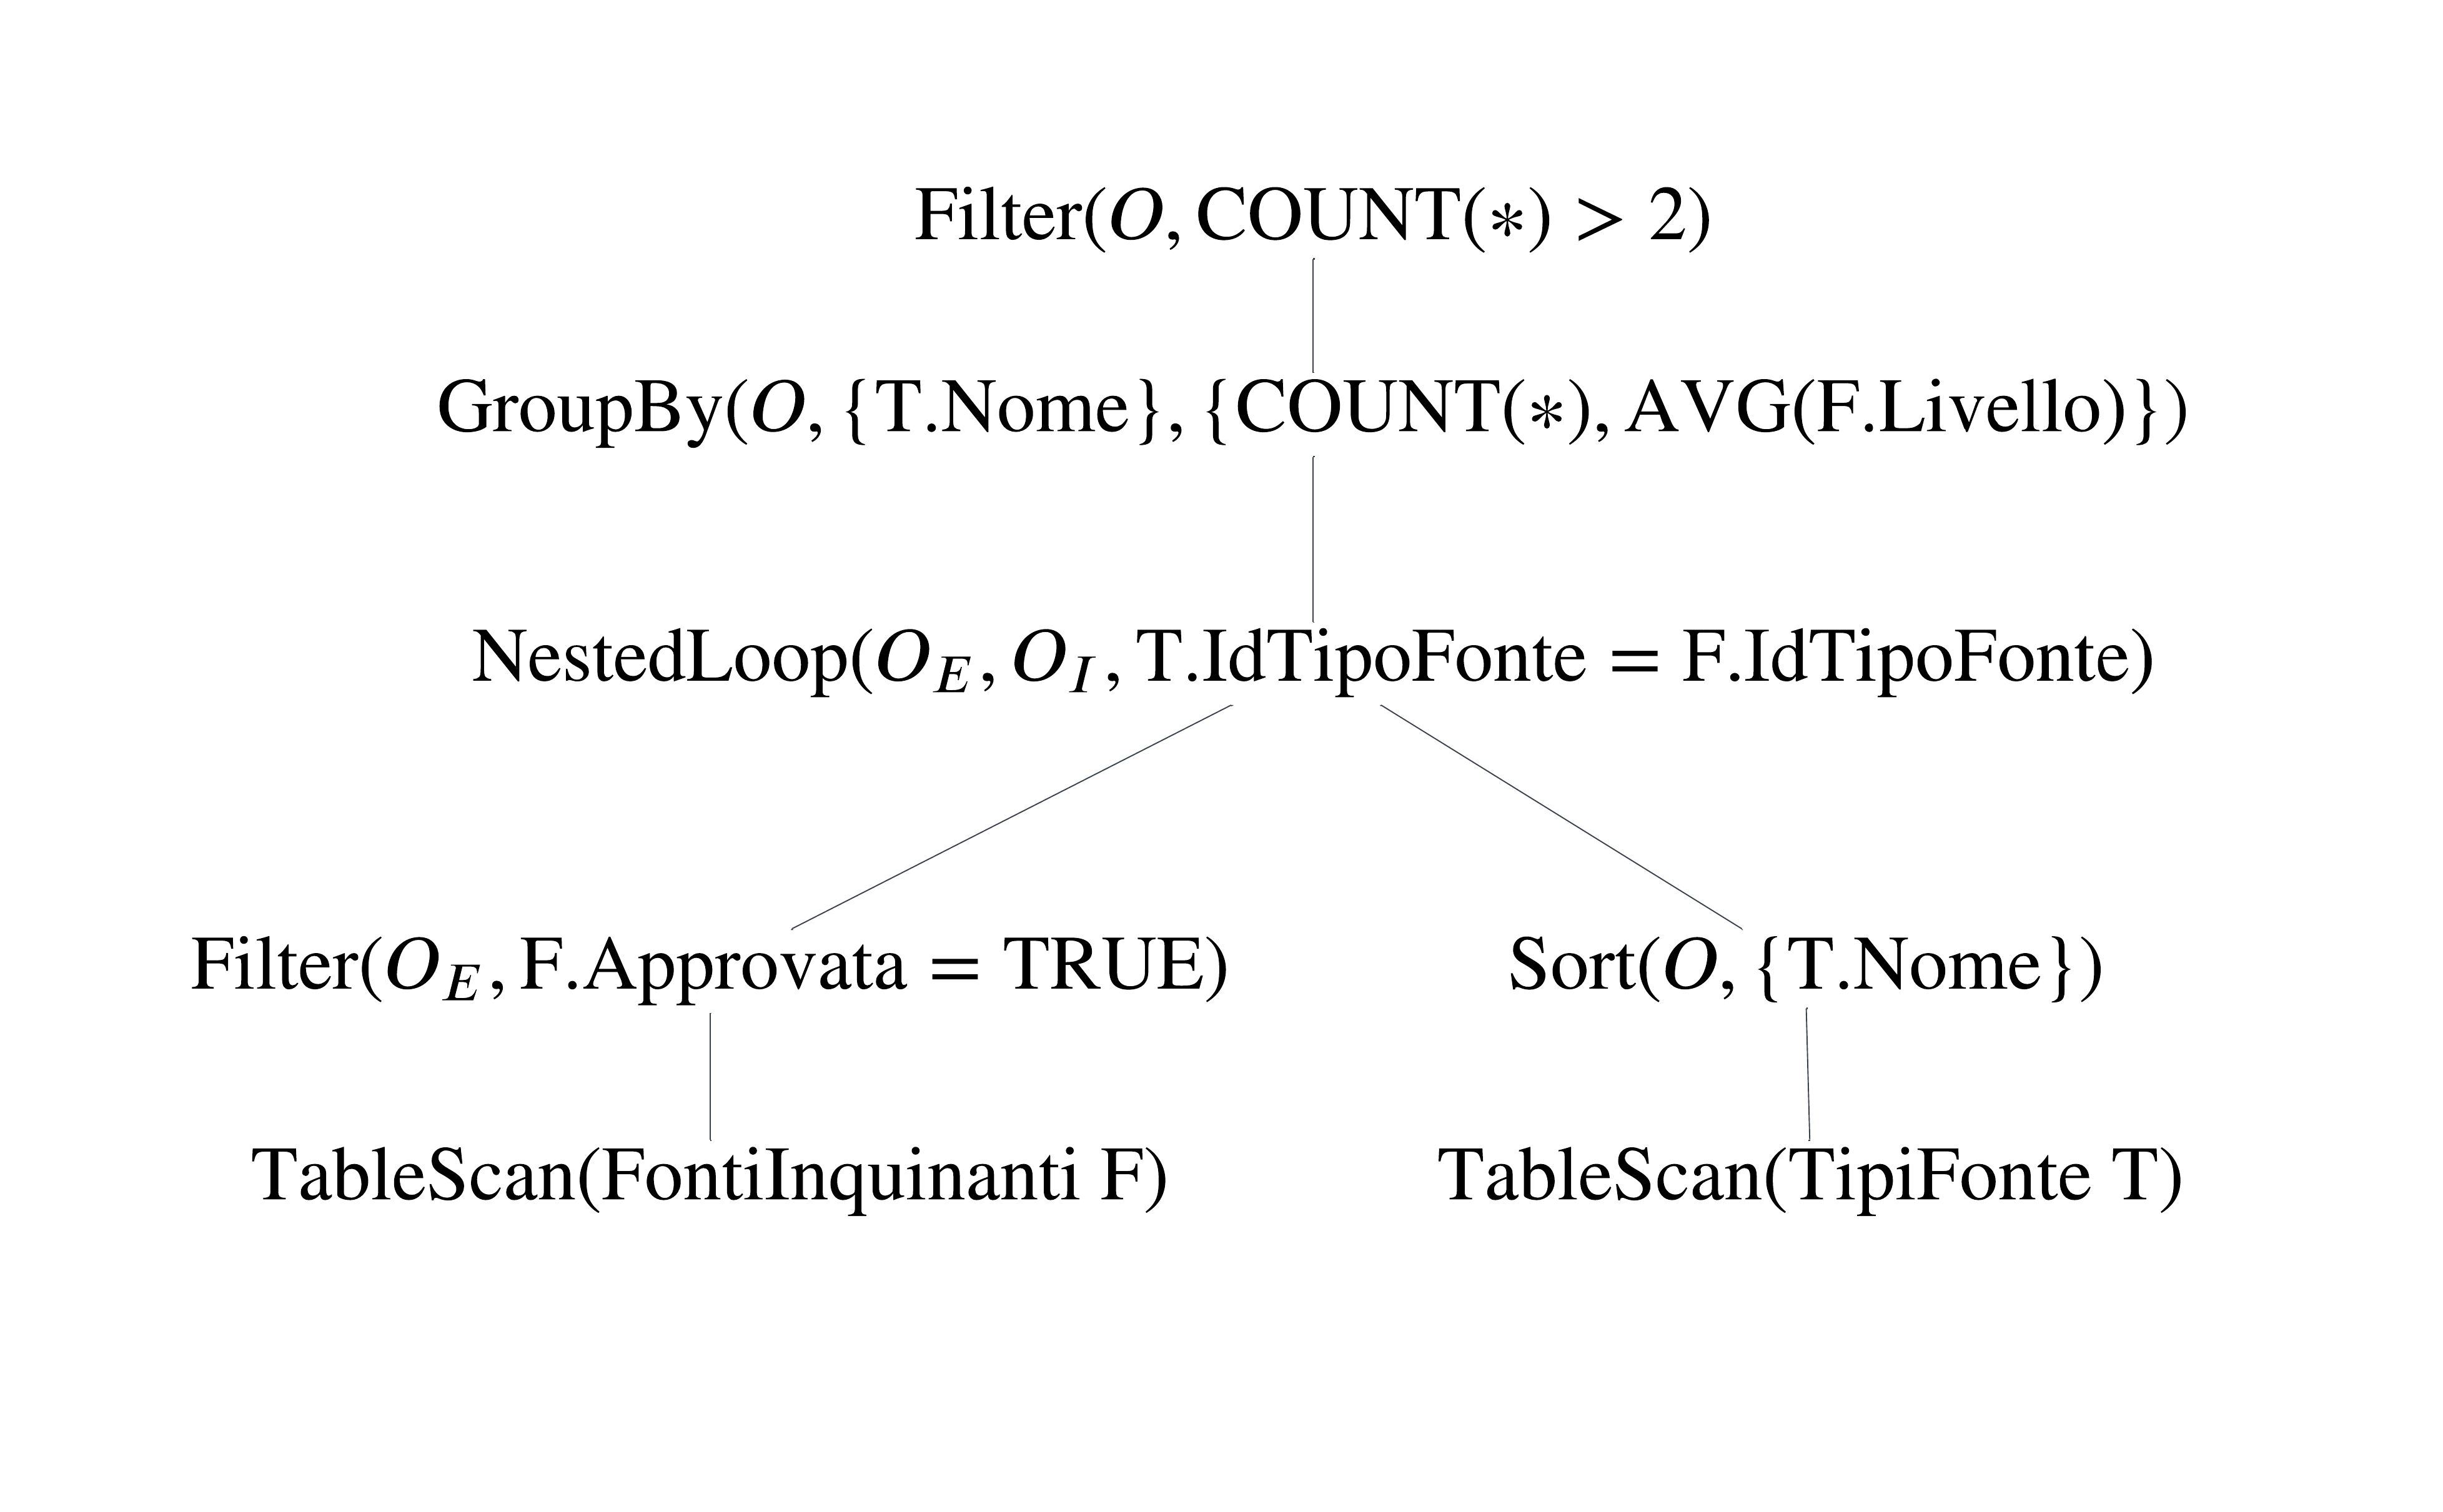
\includegraphics[scale=0.2]{2c.png}
			\captionof{figure}{Query \textit{c}}
		\end{minipage}
	\end{figure}
	\item[III.] Piani di accesso \textbf{fisico} con uso di indici
	\begin{figure}[!h]
		\centering
		\begin{minipage}{.3\textwidth}
			\centering
			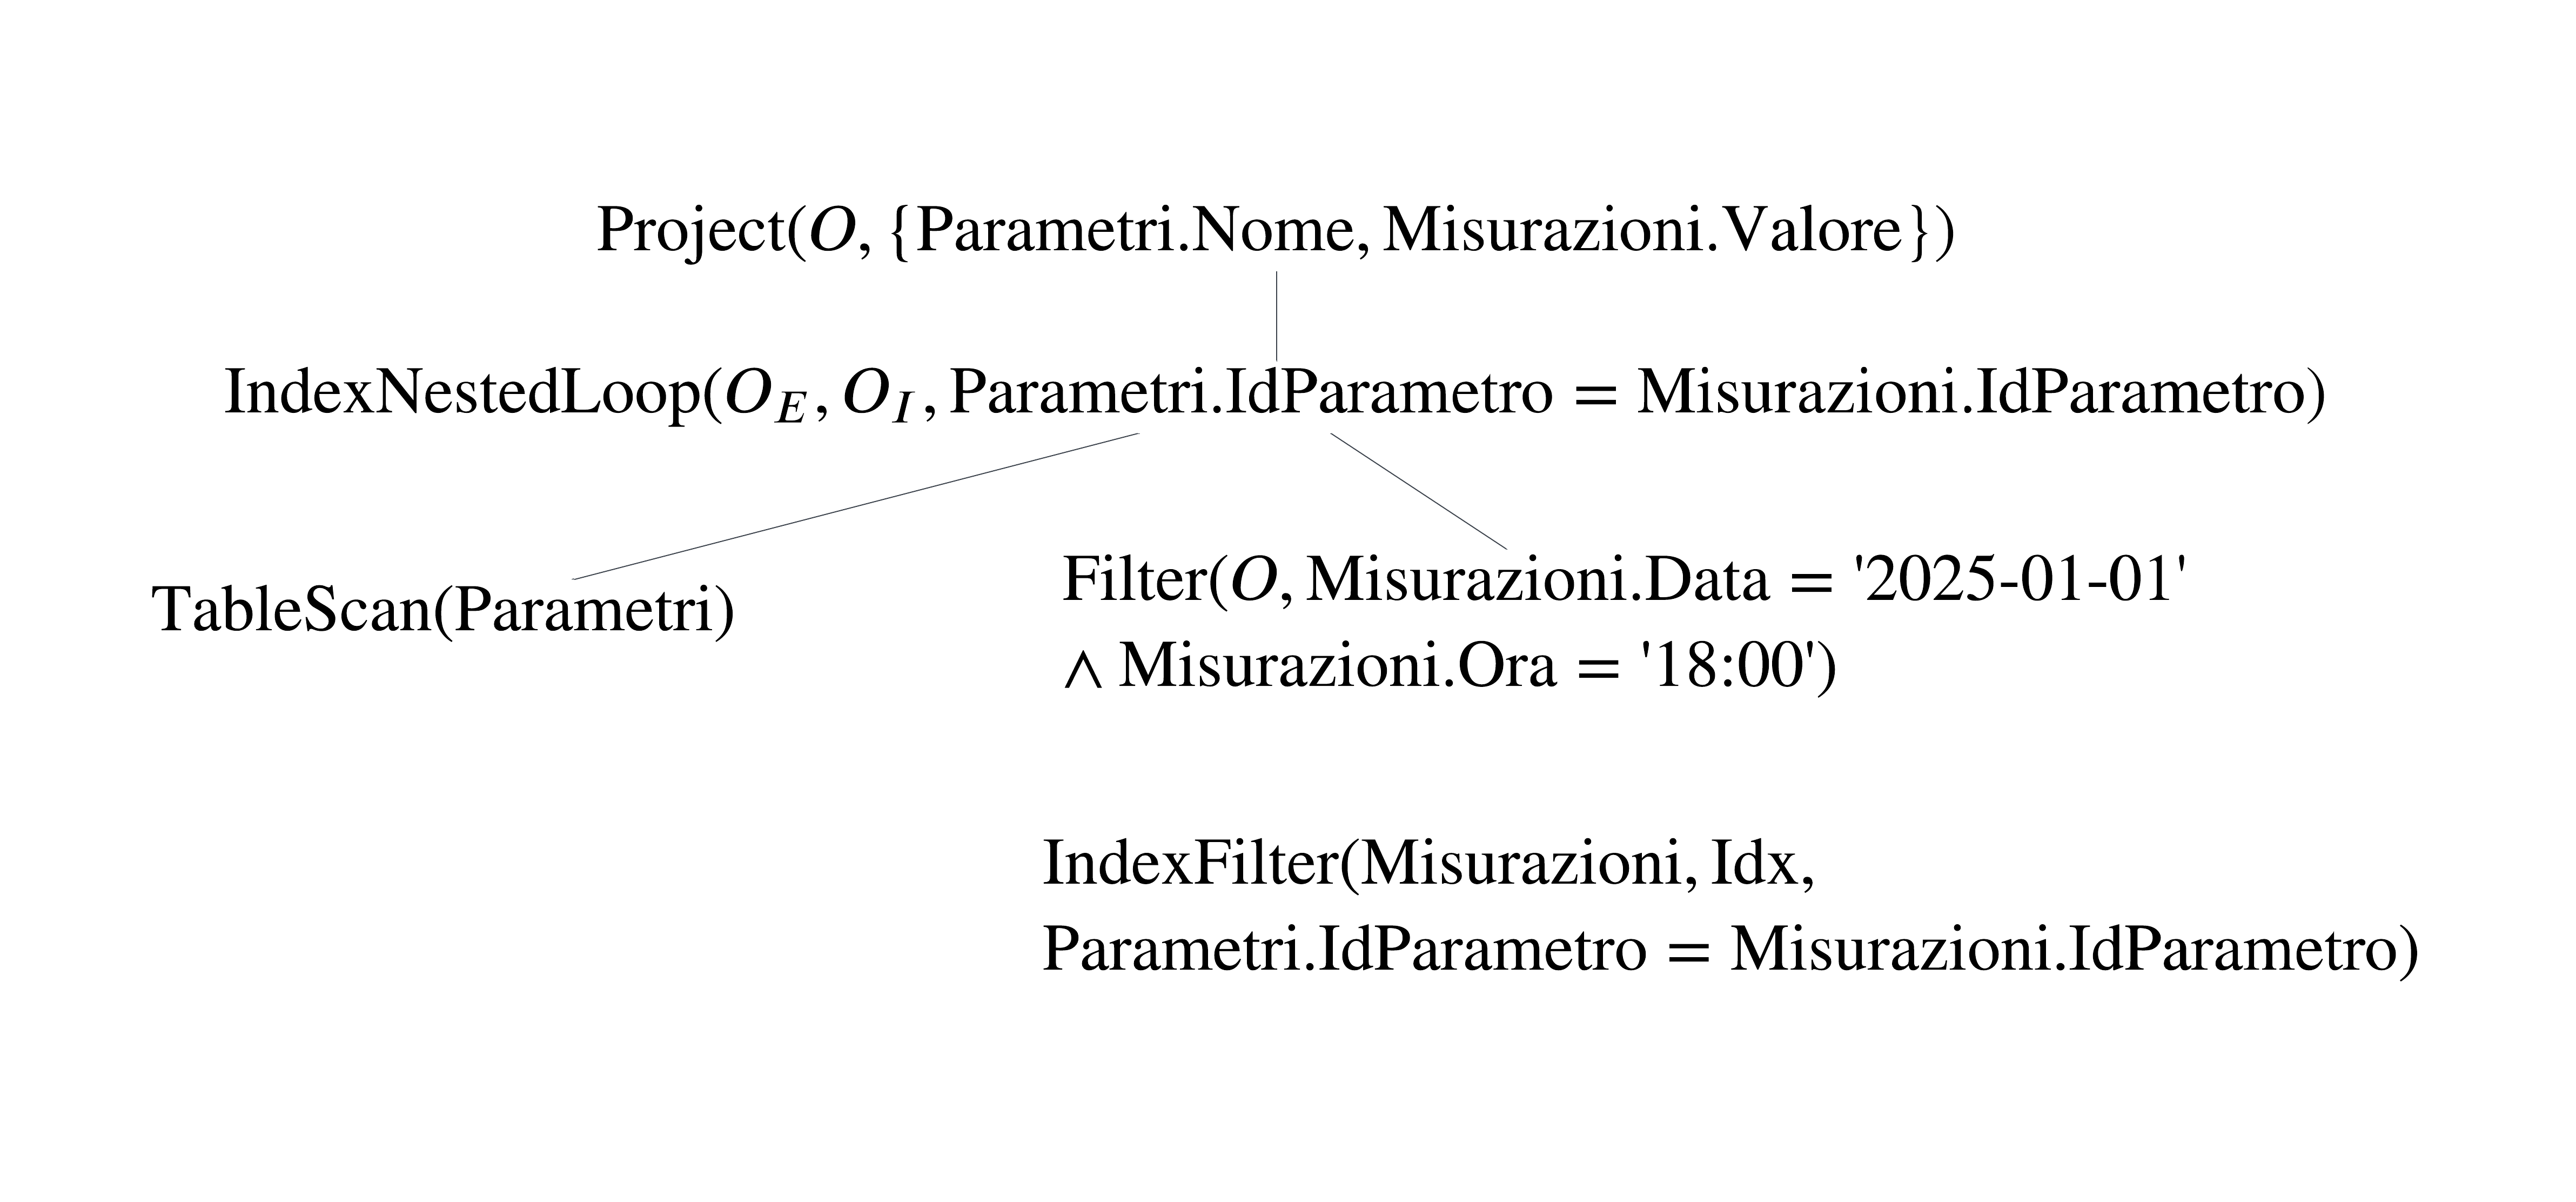
\includegraphics[scale=0.25]{3a.png}
			\captionof{figure}{Query \textit{a}}
		\end{minipage}\\
		\begin{minipage}{.3\textwidth}
			\centering
			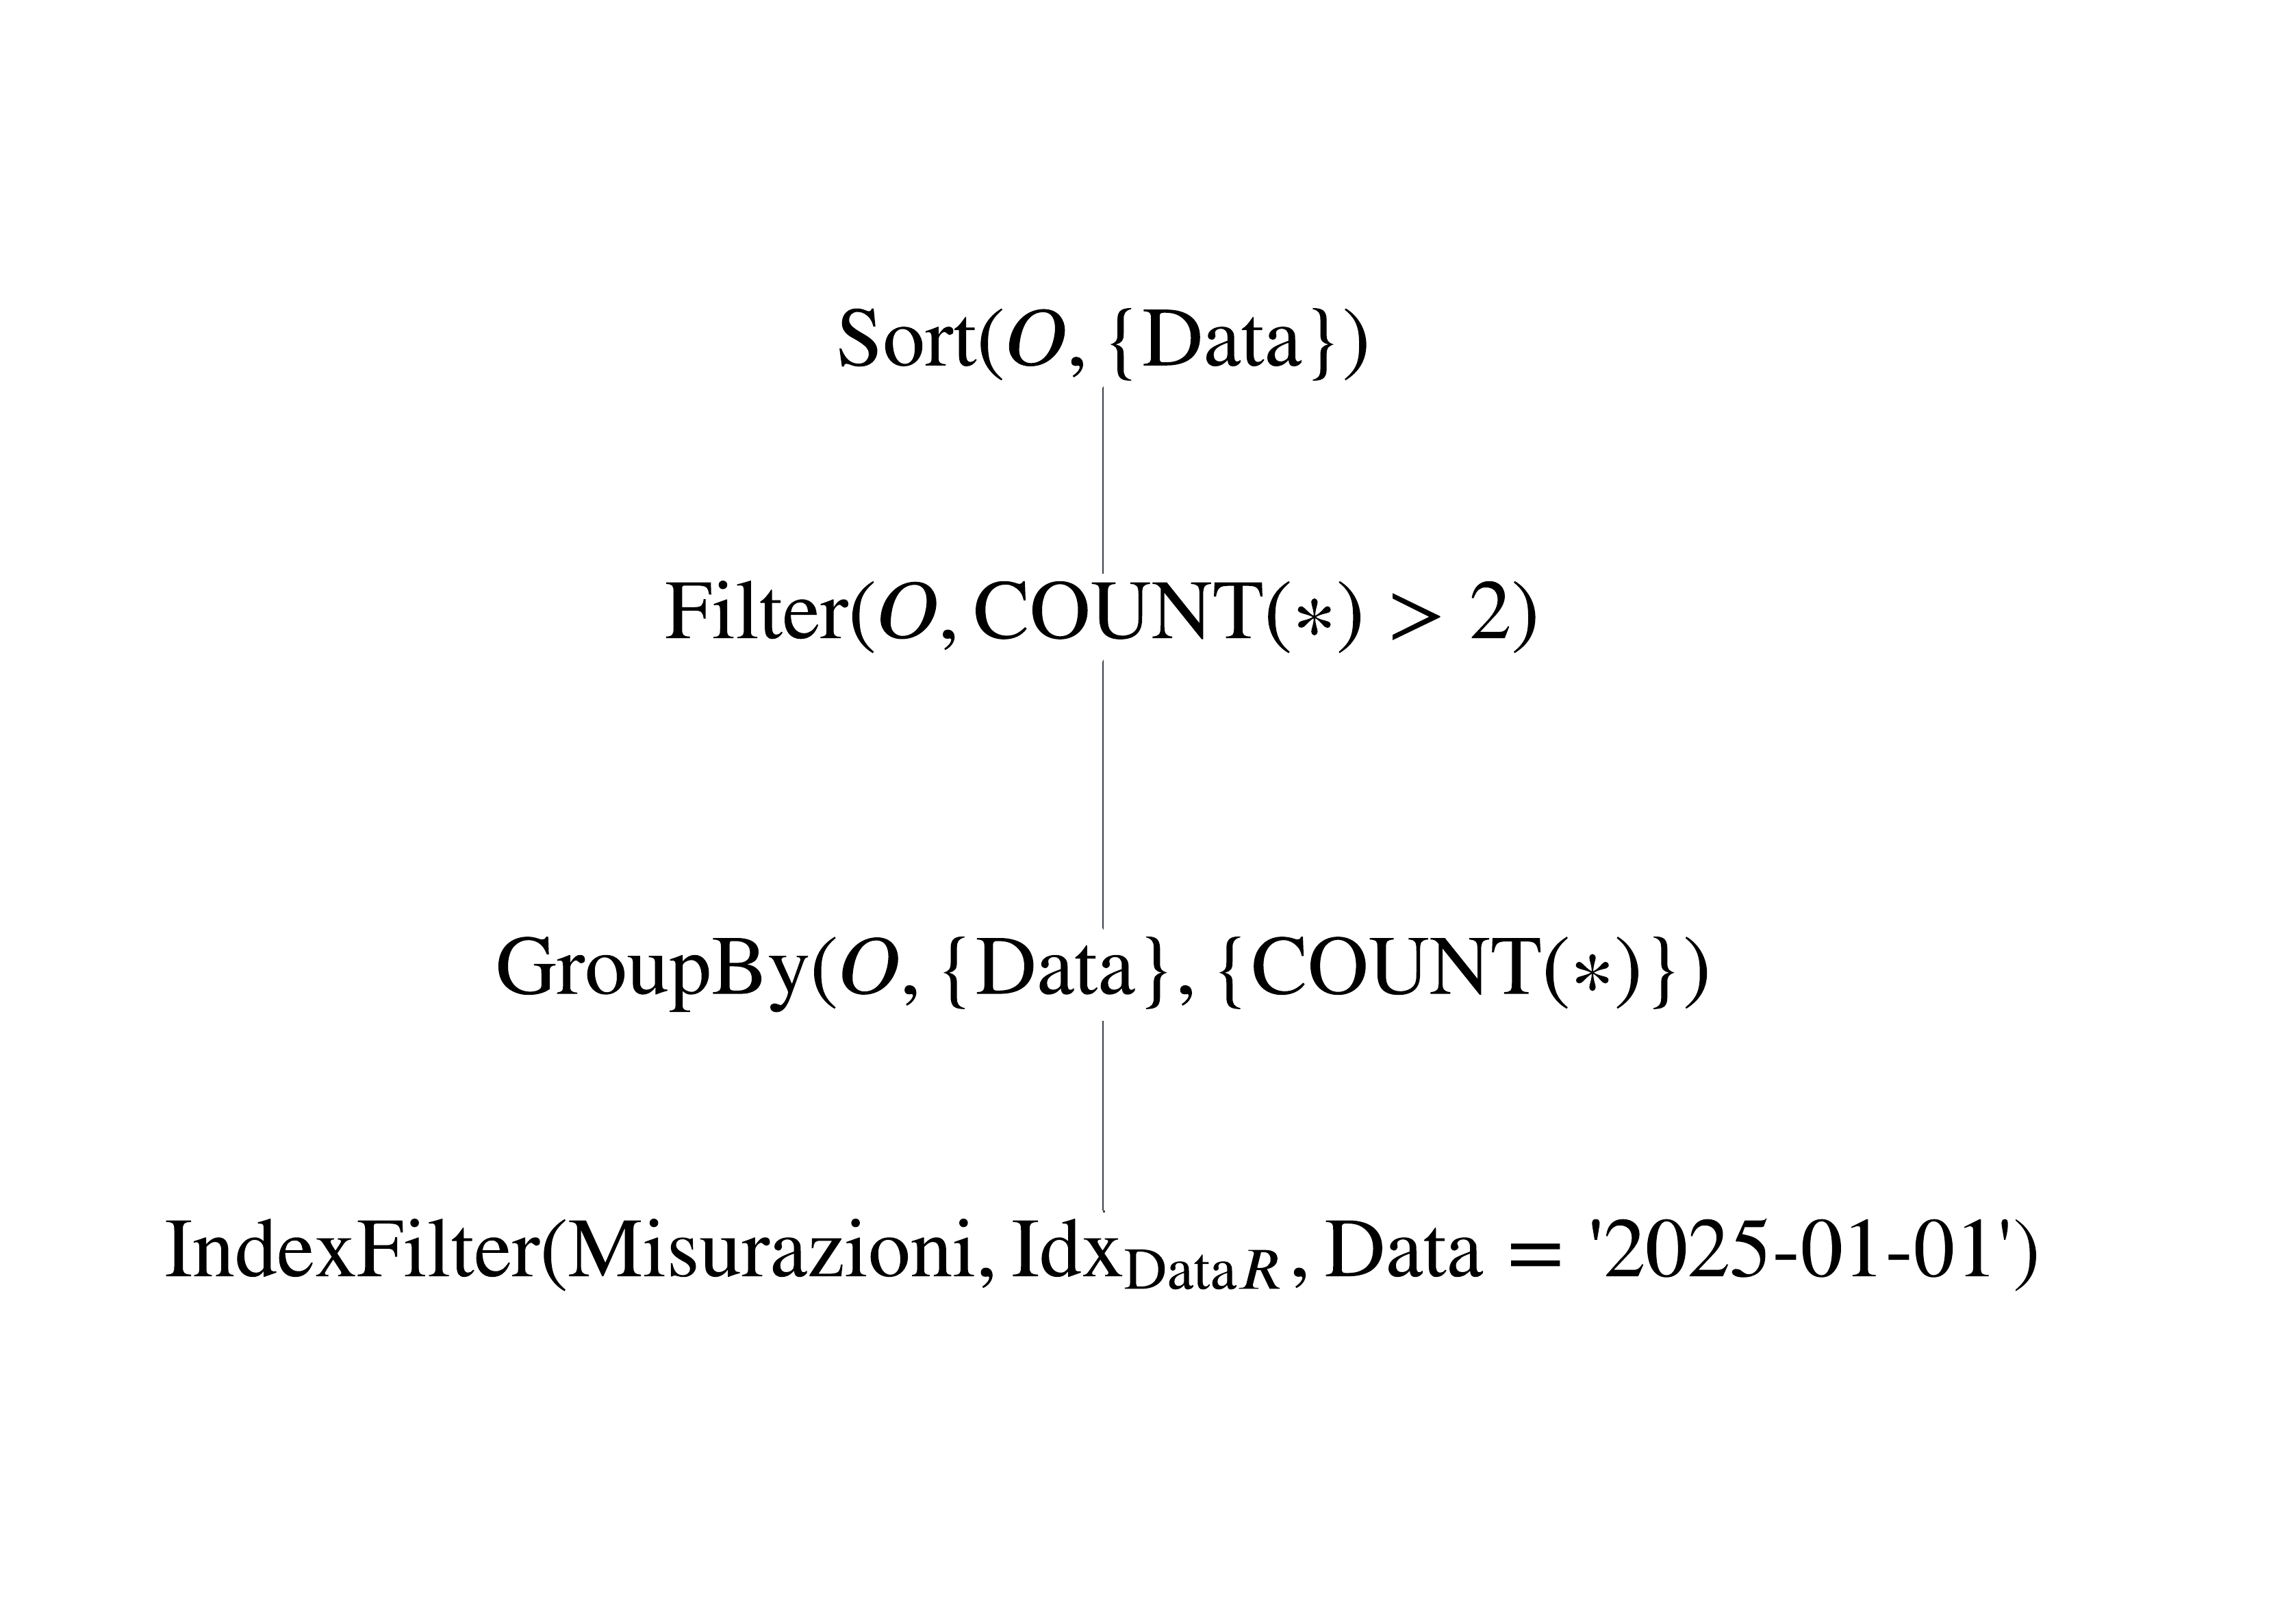
\includegraphics[scale=0.25]{3b.png}
			\captionof{figure}{Query \textit{b}}
		\end{minipage} \hspace{50pt}
		\begin{minipage}{.3\textwidth}
			\centering
			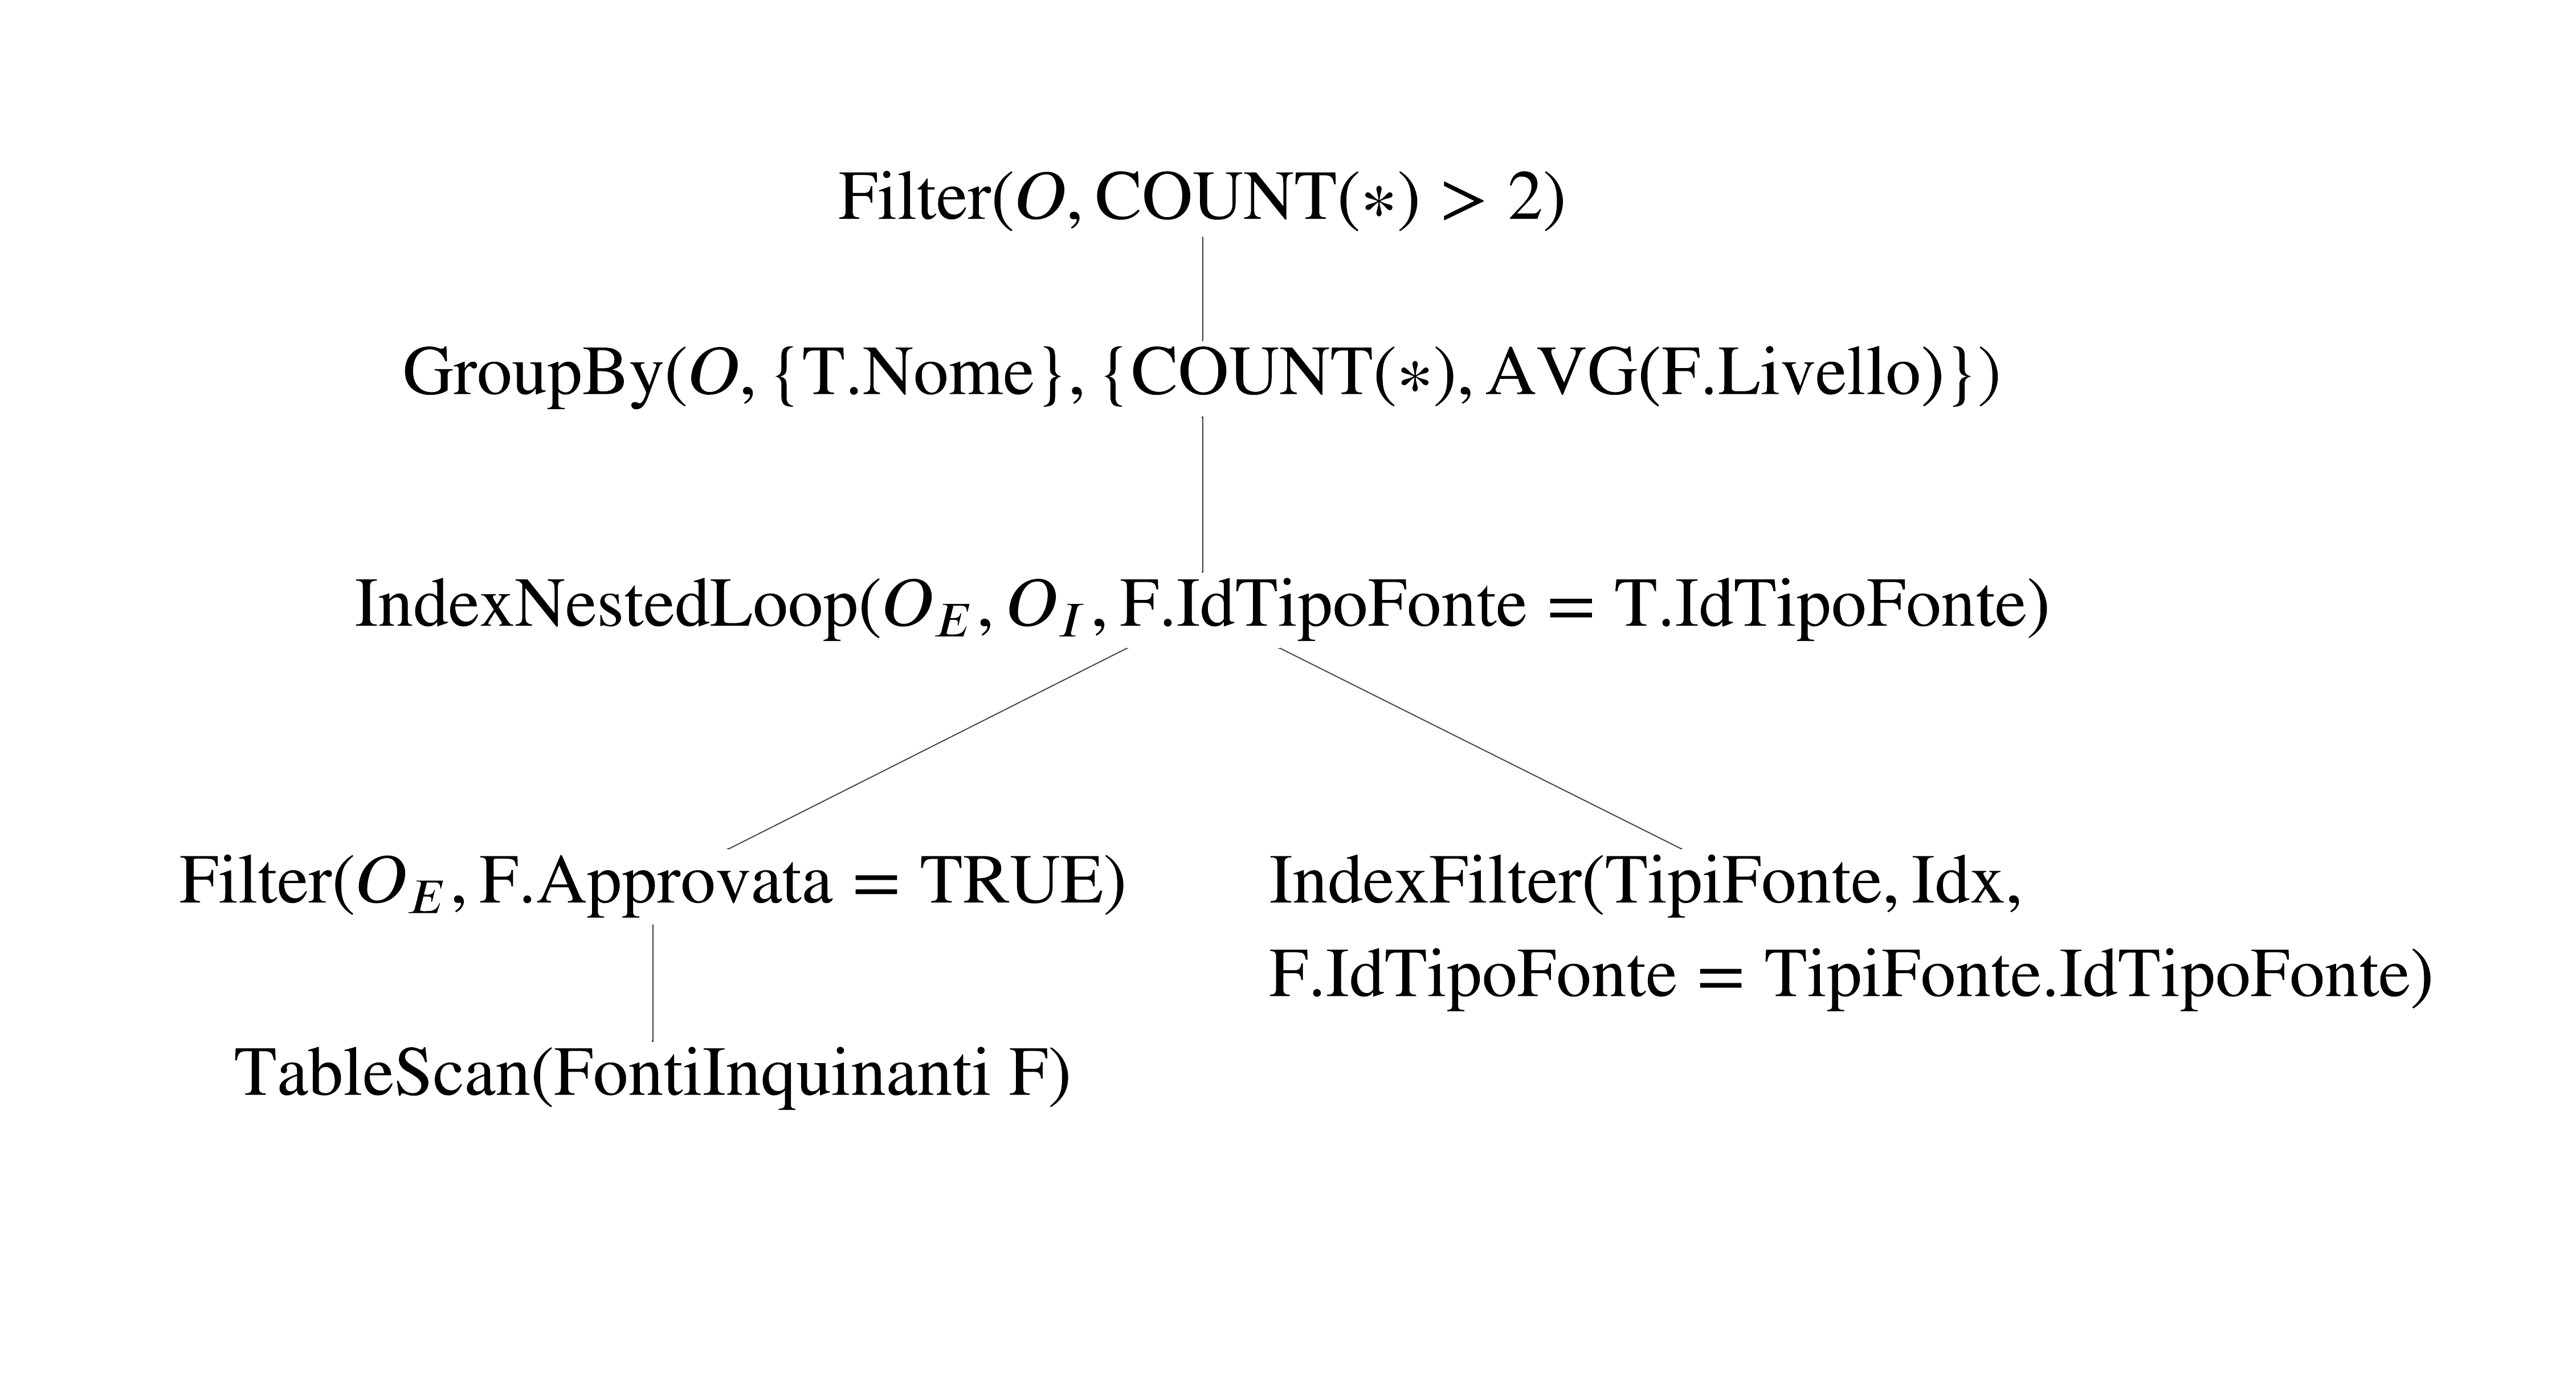
\includegraphics[scale=0.25]{3c.png}
			\captionof{figure}{Query \textit{c}}
		\end{minipage}
	\end{figure}
\end{enumerate}